%% bare_jrnl.tex
%% V1.4b
%% 2015/08/26
%% by Michael Shell
%% see http://www.michaelshell.org/
%% for current contact information.
%%
%% This is a skeleton file demonstrating the use of IEEEtran.cls
%% (requires IEEEtran.cls version 1.8b or later) with an IEEE
%% journal paper.
%%
%% Support sites:
%% http://www.michaelshell.org/tex/ieeetran/
%% http://www.ctan.org/pkg/ieeetran
%% and
%% http://www.ieee.org/

%%*************************************************************************
%% Legal Notice:
%% This code is offered as-is without any warranty either expressed or
%% implied; without even the implied warranty of MERCHANTABILITY or
%% FITNESS FOR A PARTICULAR PURPOSE! 
%% User assumes all risk.
%% In no event shall the IEEE or any contributor to this code be liable for
%% any damages or losses, including, but not limited to, incidental,
%% consequential, or any other damages, resulting from the use or misuse
%% of any information contained here.
%%
%% All comments are the opinions of their respective authors and are not
%% necessarily endorsed by the IEEE.
%%
%% This work is distributed under the LaTeX Project Public License (LPPL)
%% ( http://www.latex-project.org/ ) version 1.3, and may be freely used,
%% distributed and modified. A copy of the LPPL, version 1.3, is included
%% in the base LaTeX documentation of all distributions of LaTeX released
%% 2003/12/01 or later.
%% Retain all contribution notices and credits.
%% ** Modified files should be clearly indicated as such, including  **
%% ** renaming them and changing author support contact information. **
%%*************************************************************************


% *** Authors should verify (and, if needed, correct) their LaTeX system  ***
% *** with the testflow diagnostic prior to trusting their LaTeX platform ***
% *** with production work. The IEEE's font choices and paper sizes can   ***
% *** trigger bugs that do not appear when using other class files.       ***                          ***
% The testflow support page is at:
% http://www.michaelshell.org/tex/testflow/



\documentclass[journal,article,submit,pdftex,moreauthors]{Definitions/mdpi}

\usepackage{amsmath}
\usepackage{ifthen}
\usepackage[dvipsnames]{xcolor}
\usepackage{graphicx}
\usepackage{float}
\usepackage{overpic}
\usepackage{subcaption}
\usepackage{placeins}
\usepackage{booktabs, longtable, multirow, array, makecell}

%\usepackage{lipsum}
%\usepackage{cite}
\input{localdefs}

% --- Patch: make \address append (not overwrite), so multiple affiliations show ---
\makeatletter
\providecommand\@address{}%
\renewcommand\address[2][]{%
  \g@addto@macro\@address{\par\noindent\textsuperscript{#1}#2\par}%
}
\makeatother

% correct bad hyphenation here
% \hyphenation{op-tical net-works semi-conduc-tor}


% ------------ MDPI Front Matter ------------
\Title{Machine Learning Based Static Performance Prediction of Bonded Structural Patch Repairs}

\Author{
  Yesim Kokner $^{1,*}$,
  M. Umit Uyar $^{2}$,
  Feridun Delale $^{1}$,
  Niell Elvin $^{1}$,
  Hasan S. Kayman $^{2}$
}

% These two lines help the class populate headers/metadata correctly
\AuthorNames{Kokner, Y.; Uyar, M.U.; Delale, F.; Elvin, N.; Kayman, H.S.}
\AuthorCitation{Kokner, Y.; Uyar, M.U.; Delale, F.; Elvin, N.; Kayman, H.S.}

\address[1]{\quad Department of Mechanical Engineering, The City College of New York, New York, NY 10031, USA}
\address[2]{\quad Department of Electrical Engineering, The City College of New York, New York, NY 10031, USA}


% Corresponding author(s)
\corres{* Correspondence: ykokner@ccny.cuny.edu}

\abstract{This study investigates adhesively bonded composite patch repair to enhance the load-carrying capacity of damaged metallic structures, introducing a novel FE-augmented machine learning (ML) framework that addresses the limited availability of experimental data in structural repair applications. To evaluate this approach, aluminum and steel specimens with central fatigue cracks were repaired using glass-fiber/epoxy and carbon-fiber/epoxy composite patches and tested under quasi-static loading at room (70$^\circ$F), high (145$^\circ$F), and low (-60$^\circ$F) temperatures. Finite element (FE) models were then developed in ABAQUS© to predict the failure loads of the patched specimens under varying temperature conditions, showing excellent agreement with the experimental data. The high accuracy of the FE predictions enabled their use as additional training data, effectively augmenting the limited experimental dataset and allowing the development of more robust regression models. Ten Machine Learning (ML) regression models---linear regression (LR), polynomial regression (PR), support vector regression (SVR), random forest (RF), gradient boosting (GB), XGBoost (XGB), LightGBM (LGBM), Gaussian process (GP) regression, artificial neural networks (ANNs), and Kolmogorov--Arnold networks (KANs)---were trained to predict the failure load of both unpatched and patched specimens as a function of material type, temperature, specimen thickness, crack length, and, for patched specimens, patch type and thickness. The datasets combined a limited set of physical results (75 patched samples: 63 experimental and 12 finite-element; 72 unpatched samples: 27 experimental and 45 theoretical) with Gaussian-mixture-model synthetic samples used only to augment the training data up to 300 samples per case. Using a leakage-free protocol in which synthetic data are generated inside each cross-validation fold and models are evaluated on an untouched hold-out set of real data, the best hold-out regression models achieved mean absolute percentage errors of 3.73\% (SVR, patched, $R^2=0.937$) and 3.18\% (XGBoost, unpatched, $R^2=0.994$), while the ANN remained competitive (5.81\%, $R^2=0.874$ and 5.37\%, $R^2=0.981$, respectively). By combining experimental testing, FE simulations, and regression-based predictive modelling, this study provides a novel, data-efficient framework for predicting the performance of adhesively bonded composite patch repairs under varying thermal and mechanical conditions.}

\keyword{composite patch repair; adhesively bonded repair; fatigue crack; static failure load prediction; temperature effects;  finite element analysis (FEA); machine learning (ML)}

% -------------------------------------------------------

% The paper headers
\markboth{Journal of TBD} {Name \MakeLowercase{\textit{et al.}}: A Comparative Study of ML Model}
% The only time the second header will appear is for the odd numbered pages
% after the title page when using the twoside option.
% 
% *** Note that you probably will NOT want to include the author's ***
% *** name in the headers of peer review papers.                   ***
% You can use \ifCLASSOPTIONpeerreview for conditional compilation here if
% you desire.

% If you want to put a publisher's ID mark on the page you can do it like
% this:
%\IEEEpubid{0000--0000/00\$00.00~\copyright~2015 IEEE}
% Remember, if you use this you must call \IEEEpubidadjcol in the second
% column for its text to clear the IEEEpubid mark.

% use for special paper notices
%\IEEEspecialpapernotice{(Invited Paper)}

% For peer review papers, you can put extra information on the cover
% page as needed:
% \ifCLASSOPTIONpeerreview
% \begin{center} \bfseries EDICS Category: 3-BBND \end{center}
% \fi
%
% For peerreview papers, this IEEEtran command inserts a page break and
% creates the second title. It will be ignored for other modes.

\makeatletter\providecommand{\@datepublished}{}\makeatother
\setcounter{page}{1}

\pubyear{2024}
\copyrightyear{2024}
\articlenumber{0}

\begin{document}
\section{Introduction}

Adhesively bonded composite patch repair is a practical temporary method to restore the structural performance of damaged components in aircraft and vehicles, allowing continued operation until permanent repair or replacement can be performed. This approach offers improved load transfer, higher fatigue resistance, and improved corrosion resistance compared to traditional mechanical fastening techniques. Despite these advantages, predicting the performance of bonded repairs under varying environmental and mechanical conditions remains challenging. The performance of repaired structures depends on several interacting parameters, including substrate material, adhesive properties, patch configuration, and temperature, all of which can influence load transfer across the bonded interface.
Composite patches offer high strength-to-weight ratios, improved corrosion resistance, and adaptability to complex geometries, making them attractive candidates in aerospace, automotive, and civil engineering applications \cite{Mohammadi,Schubbe,Tavakkolizadeh}. Unlike traditional mechanical fastening methods, bonded repairs reduce stress concentrations and help prevent further damage near fastener holes. In addition, bonded repairs redistribute stresses and slow crack growth, thus extending the fatigue life of damaged metal structures\cite{Rhys,JonesR}. The effectiveness of bonded composite repairs depends on factors such as patch and substrate types and thicknesses, adhesive properties, surface preparation, and curing conditions \cite{Repair}. 

The influence of patch and substrate thickness on structural performance has been widely examined in the literature. Researchers in \cite{Hosseini} demonstrated that the effectiveness of bonded repairs is strongly dependent on the thickness of the panel: while thin panels exhibited a 236\% increase in crack growth life using a 16-layer patch, thick panels showed only a 23-55\% improvement with a 4-layer patch.
Similarly, the experimental study in \cite{Sohail} on 2024-T3 aluminum plates repaired with carbon/epoxy patches (4, 6 and 8 plies) reported that fatigue life improved with increasing patch thickness, reaching nearly a threefold improvement with 8 plies. However, they emphasized that excessive patch stiffness can lead to new stress concentrations, highlighting the need for optimal patch thickness selection. Xiong and Shenoi \cite{Xiong} also confirmed that patch thickness significantly affects both static and fatigue strength, whereas the fiber-reinforced composite material primarily governs fatigue performance. In addition to patch thickness, substrate thickness significantly influences crack growth behavior. Broek and Schijve \cite{Broek} demonstrated that cracks propagate more rapidly in thicker substrates, indicating a strong relationship between substrate thickness and crack growth rate. Furthermore, Kan and Ratwani \cite{Kan} found that specimens with greater thickness (6.4 mm) exhibited shorter crack growth lives compared to those with thinner thickness (3.1 mm), emphasizing the critical importance of both patch and substrate thickness in bonded composite repairs. 

Another important design aspect in bonded repair applications is the patch configuration.
Experimental studies \cite{Srilakshmi,Ramji,Liu,LiL,Günther} have compared single and double-sided repair schemes and shown that double-sided repairs typically result in superior mechanical performance. Compared to unrepaired specimens, single-sided repairs increase ultimate load capacity by approximately 7\%, whereas double-sided configurations provide around 12\% higher strength and nearly double the fatigue life due to a greater reduction in stress intensity factors. However, when accessibility to both sides of the structure is limited, single-sided repairs remain a practical and effective solution. Considering these findings and accessibility limitations, this study employed a single-sided repair configuration to simulate realistic field repair conditions.

Bonded composite repair has been established as a reliable method for restoring structural integrity in aging metallic components. However, its effectiveness is significantly affected by environmental conditions. Near the adhesive’s glass transition temperature, both stiffness and bond strength decrease, whereas at low temperatures, the adhesive becomes more brittle. Our previous studies \cite{Kokner,Yesim} demonstrated that bonded repairs on Aluminum 6061 and A36 steel enhance load capacity at room and low temperatures, but their efficiency declines at elevated temperatures due to adhesive softening. Accurately predicting the performance of bonded repairs under these varying conditions remains a significant challenge.

In addition to the experimental investigations, several numerical studies have been conducted using the finite element method (FEM) to analyze the behavior of cracked metallic structures repaired with bonded composite patches. In previous studies, finite element analyses showed that patch geometry, adhesive properties, patch configuration, and material type significantly influence stress distribution, load transfer, and crack propagation behavior. Analyses focusing on patch thickness and geometry show that increasing patch thickness or width reduces the stress intensity factor (SIF) and delays crack growth, while excessive adhesive thickness or stiffness limits load transfer and decreases repair efficiency \cite{Papanikos,BouiadjrA,Gunes,Achour}. Adhesive thickness was also found to be a key factor influencing repair efficiency. Studies reported that thinner adhesive layers enhance stress transfer between the patch and substrate, leading to lower stress intensity factors and improved fatigue life, whereas thicker adhesive layers reduce load transfer and lower the overall repair efficiency \cite{Walde}. Belhouari et al.\cite{Serier} demonstrated that double-sided symmetric patches achieve higher SIF reduction and alleviate bending effects typically observed in single-sided repairs, leading to more balanced stress distributions. In \cite{Ouinas}, the influence of composite patch material and fiber orientation was investigated, and it was shown that boron epoxy patches outperform graphite epoxy alternatives, while fibers oriented perpendicular to the crack path enhance SIF reduction by more than 50\%. Three-dimensional finite element models have improved prediction accuracy by capturing out-of-plane deformations and complex stress states near the crack front, overcoming the limitations of simplified two-dimensional analyses \cite{Ripi}. Overall, the findings demonstrate that finite element modeling (FEM) is a critical method for optimizing patch geometry, adhesive selection, and configuration to improve the structural integrity and durability of bonded composite repairs.

Although finite element modeling offers significant insight into the mechanical response of bonded repairs, recent developments in data-driven approaches, particularly ANNs and modern regressors, have facilitated more efficient prediction of fatigue and damage behavior. ANNs and modern regressors have emerged as effective data-driven tools for predicting fatigue life and modeling crack propagation in structural materials.
In contrast to conventional S-N curves or fracture mechanics-based methods, ML models can capture nonlinear interactions among multiple influencing factors, including material properties, crack geometry, loading conditions, and environmental effects.
Recent studies \cite{Alkunte} and \cite{magliacano2026element} utilized ANN and other machine learning models to predict the fatigue life of functionally graded materials, demonstrating strong agreement between predicted and experimental results. In \cite{Rohman}, an ANN-based model demonstrated reliable predictions of fatigue life for composite materials under variable amplitude loading. In addition, ANN models have achieved accurate fatigue life estimation for multidirectional glass fiber-reinforced laminates \cite{Vassilopoulos} and for various composite systems using alternative machine learning approaches such as polynomial classifiers \cite{Kadi}. In \cite{Mishra}, a multilayer feedforward ANN successfully predicted the low-cycle fatigue life of Al-Si-Mg alloys, identifying key material and processing parameters influencing fatigue performance. A hybrid approach combining ANN with finite element models further improved repair evaluation accuracy and reduced experimental effort in composite patch repairs \cite{Zhang}. Moreover, ANNs have been applied to efficiently predict fracture mechanics parameters such as the J-integral from finite element results \cite{Mortazavi}. Recent work has further demonstrated that ANN models trained using finite element-derived fracture parameters can accurately predict mixed-mode fracture loads, outperforming conventional linear elastic fracture criteria while significantly reducing experimental effort \cite{Bahrami2023ANNFracture}. These previous studies have shown that machine learning techniques can improve prediction accuracy and reduce experimental requirements when assessing the fatigue and damage behavior of bonded composite repairs. In light of these findings, this study combines experimental data with finite-element modeling results to develop a machine-learning-based method for predicting the static performance of bonded structural patch repairs in different environmental conditions.


\section{Experimental Methodology}
\label{sec:setup}
\subsection{Materials}
Two substrate materials were selected for this study: Al 6061 and A36 steel. Al 6061 specimens were prepared in two thicknesses, 1/8 inch (3.18 mm) and 0.190 inches (4.83 mm), while A36 steel specimens were 1/8 inch (3.18 mm) thick. Each specimen was machined with a central 0.19-inch notch, followed by fatigue loading to produce 0.05-inch cracks on each side of the notch, resulting in a total crack length of $2a=0.29$ inches. The configuration and dimensions of the unpatched specimens are presented in Figure~\ref{fig:1}.
\begin{figure}[h]
    \centering
    \includegraphics[width=1\textwidth]{Figures/Fig1.pdf}
    \centering
    \caption{\centering Schematic representation of the unpatched specimens, showing (a) the overall geometry, (b) the notch and fatigue crack region, and (c) detailed dimensions of the notch geometry.}
    \label{fig:1}
\end{figure}


\newpage The composite patches were fabricated in-house using the vacuum infusion process. Two glass-fiber/epoxy panels with thicknesses of 1.0 mm and 1.64 mm, as well as a carbon-fiber/epoxy patch of approximately 0.89 mm, were produced from unidirectional fiber fabrics. Surface preparation to ensure strong adhesion was applied exclusively to the metallic substrates, involving acetone cleaning, sandblasting with 54-60 grit alumina oxide at 80-100 psi, and debris removal using compressed gas. The patches were bonded with Hysol EA 9309NA, a two-part aerospace-grade epoxy adhesive, and oven-cured at 66$^\circ$C for 1 hour. Testing was conducted after a 48-hour post-cure period. The configuration and fiber orientation of the patched specimens are presented in Figure~\ref{fig:geometry}. Fibers were aligned perpendicular to the crack direction to maximize load transfer.
\begin{figure}[h]
    \centering
    \includegraphics[width=1\textwidth]{Figures/Fig2.jpg}
    \centering
    \caption{\centering Schematic of the patched specimen subjected to tensile loading. The composite patch is bonded over the crack region in the substrate. The inset shows the fiber orientation and the crack length (2a) within the patched area.}
    \label{fig:geometry}
\end{figure}

\subsection{Experimental Setup}
Static tensile tests were conducted to evaluate the load-carrying capacity of both patched and unpatched specimens. All specimens featured a central crack ($a$ = 0.145 inches) and were loaded to failure using a universal Instron testing machine at a constant crosshead speed of 2 mm/min. The testing was performed at three temperatures: room temperature (70$^\circ$F), high temperature (145$^\circ$F), and low temperature (-60$^\circ$F), using an environmental chamber. Specimens were exposed for at least 30 minutes at the target temperature to achieve thermal equilibrium. The temperature was monitored using thermocouples attached to both the patched specimens and the chamber. Force and displacement data were collected, and patch performance was assessed by comparing failure loads of patched and unpatched specimens. 

\subsection{Experimental Results}
Unpatched specimens made of A36 steel with a thickness of 1/8 inch and Al 6061 with thicknesses of 1/8 inch and 0.190 inches were tested to establish the reference performance of the cracked substrates prior to patch application. Each specimen contained a central crack with a half-length of 0.145 inches. After determining the reference performance, identical cracked specimens were repaired using glass fiber/epoxy composite patches with thicknesses of 1.0 mm and 1.64 mm and carbon fiber/epoxy composite patches with an approximate thickness of 0.89 mm. The repaired specimens were then tested under the same loading conditions at three temperature levels: room-temperature (70$^\circ$F), high-temperature (145$^\circ$F), and low-temperature (-60$^\circ$F), to evaluate the effectiveness of the bonded patches relative to the unpatched specimens. Force-displacement curves for the unpatched, glass-fiber (GF) patched, and carbon-fiber (CF) patched Al 6061 specimens with a thickness of 1/8 inch are shown in Figure~\ref{fig:Fig3}, while the complete set of results obtained under different environmental conditions is summarized in Table~\ref{tab:failureloads}. Similar static tests were also performed on A36 steel unpatched, GF-patched and CF-patched specimens, with the results shown also in Table~\ref{tab:failureloads}.

\begin{figure}[H]
\centering

\begin{minipage}{0.50\textwidth}
  \centering
  \begin{overpic}[width=\textwidth]{Figures/Fig3a.png}
    \put(92,82){\normalsize\textbf{(a)}}
  \end{overpic}
\end{minipage}

\vspace{0.5em}

\begin{minipage}{0.50\textwidth}
  \centering
  \begin{overpic}[width=\textwidth]{Figures/fig3b.png}
    \put(92,82){\normalsize\textbf{(b)}}
  \end{overpic}
\end{minipage}

\vspace{0.5em}

\begin{minipage}{0.50\textwidth}
  \centering
  \begin{overpic}[width=\textwidth]{Figures/fig3c.png}
    \put(92,82){\normalsize\textbf{(c)}}
  \end{overpic}
\end{minipage}

\caption{
Force-displacement curves for Al 6061 specimens with 1/8-inch thickness tested at room temperature:  
\textbf{(a)} unpatched specimen,  
\textbf{(b)} GF-patched specimen,  
\textbf{(c)} CF-patched specimen.
}
\label{fig:Fig3}
\end{figure}

To assess the influence of adherend thickness on repair performance, tensile tests were conducted on both thin and thick Al 6061 specimens. In addition, to further investigate how increased patch thickness affects the static response of repaired aluminum structures, thick Al 6061 specimens were tested using a thicker glass-fiber/epoxy composite patch. In this configuration, 1.64 mm-thick patches were used instead of 1 mm patches. These results are also summarized in Table~\ref{tab:failureloads}. At least three specimens were tested for each configuration, and in some configurations, four specimens were tested to ensure the consistency of the experimental results. The failure loads reported in Table~\ref{tab:failureloads} represent the mean values obtained from the experimental tests. Since the number of specimens for each configuration was limited, standard deviations were not calculated. All experimental results were used individually in the machine learning regression model rather than being averaged.

Static tensile tests on thin and thick Al 6061 and on A36 steel specimens showed that applying bonded patches significantly improved the load-carrying capacity at room temperature, demonstrating the repair method's effectiveness. While performance decreased at high temperature due to adhesive softening near the glass transition temperature ($T_g = 63^\circ\mathrm{C} \approx 145.4^\circ\mathrm{F}$ \cite{delale2019}), the repairs remained effective at low temperatures. Although the adhesive became more brittle under low-temperature conditions, the failure loads of the patched specimens were only slightly lower than those at room temperature, and no significant change in the failure mode was observed. This temperature-dependent behavior was consistent across all patched configurations. Increasing the patch thickness from 1 mm to 1.64 mm further improved repair efficiency, indicating that patch thickness plays an important role in overall repair performance. In contrast, changes in temperature had little effect on the unpatched specimens.

\begin{table}[H]
\centering
\caption{Critical failure loads ($P_{\mathrm{cr}}$) of unpatched, GF-patched, and CF-patched specimens under different temperature conditions.}
\label{tab:failureloads}
\begin{tabular}{p{3cm} c c c}
\toprule
\parbox[c][\height][c]{3cm}{\centering \textbf{Material}} 
    & \textbf{Temperature} 
    & \textbf{Configuration} 
    & \textbf{$P_{\mathrm{cr}}$ (kN)} \\
\midrule

% -------- Al 6061, t = 1/8" --------
\multirow{9}{*}{\parbox{3cm}{\centering \textbf{Al 6061}\\ \textit{$t = 1/8''$}}}
  & \multirow{3}{*}{70$^\circ$F}
      & Unpatched   & 17.1 \\
  &   & GF Patched  & 22.7 \\
  &   & CF Patched  & 22.9 \\[3pt]

  & \multirow{3}{*}{145$^\circ$F}
      & Unpatched   & 16.5 \\
  &   & GF Patched  & 19.7 \\
  &   & CF Patched  & 19.7 \\[3pt]

  & \multirow{3}{*}{-60$^\circ$F}
      & Unpatched   & 16.8 \\
  &   & GF Patched  & 20.9 \\
  &   & CF Patched  & 22.2 \\

\midrule

% -------- A36 Steel, t = 1/8" --------
\multirow{9}{*}{\parbox{3cm}{\centering \textbf{A36 Steel}\\ \textit{$t = 1/8''$}}}
  & \multirow{3}{*}{70$^\circ$F}
      & Unpatched   & 27.6 \\
  &   & GF Patched  & 34.1 \\
  &   & CF Patched  & 33.4 \\[3pt]

  & \multirow{3}{*}{145$^\circ$F}
      & Unpatched   & 27.6 \\
  &   & GF Patched  & 27.9 \\
  &   & CF Patched  & 27.5 \\[3pt]

  & \multirow{3}{*}{-60$^\circ$F}
      & Unpatched   & 26.8 \\
  &   & GF Patched  & 31.7 \\
  &   & CF Patched  & 31.8 \\

\midrule

% -------- Al 6061, t = 0.190" --------
\multirow{9}{*}{\parbox{3cm}{\centering \textbf{Al 6061}\\ \textit{$t = 0.190''$}}}
  & \multirow{3}{*}{70$^\circ$F}
      & Unpatched   & 25.6 \\
  &   & GF Patched  & 32.4 \\
  &   & CF Patched  & 32.3 \\[3pt]

  & \multirow{3}{*}{145$^\circ$F}
      & Unpatched   & 25.5 \\
  &   & GF Patched  & 27.2 \\
  &   & CF Patched  & 26.8 \\[3pt]

  & \multirow{3}{*}{-60$^\circ$F}
      & Unpatched   & 25.2 \\
  &   & GF Patched  & 30.6 \\
  &   & CF Patched  & 31.6 \\

\midrule

% -------- Al 6061 with thicker patch, t = 0.190" --------
\multirow{9}{*}{\parbox{3cm}{\centering \textbf{Al 6061}\\ \textit{$t = 0.190''$} \\
\textit{w/thicker GF-patch}\\}}

  & \multirow{2}{*}{70$^\circ$F}
      & Unpatched   & 25.6 \\
  &   & GF Patched  & 33.2 \\[3pt]

  & \multirow{2}{*}{145$^\circ$F}
      & Unpatched   & 25.5 \\
  &   & GF Patched  & 28.1 \\[3pt]

  & \multirow{2}{*}{-60$^\circ$F}
      & Unpatched   & 25.2 \\
  &   & GF Patched  & 32.7 \\

\bottomrule
\end{tabular}
\end{table}

\clearpage
\section{Finite Element Modeling of Unpatched and Patched Specimens} 
Linear finite element analyses were performed in ABAQUS©/CAE for both unpatched and patched specimens. Separate finite element models were created for the steel and aluminum specimens to closely match the experimental setup. The main difference between the two models was the substrate thickness: Al 6061 specimens were modeled at 3.15 mm, while A36 steel specimens were modeled at 3.25 mm. These thicknesses were chosen to match the actual test specimens. Other than material properties and thickness, the geometry, loading conditions, and modeling approach were the same for both materials. The goal of these simulations was to predict the static failure loads of the patched specimens under different environmental conditions. Three-dimensional models of the specimens which included both the notch and the pre-existing crack were created, as shown in Figure~\ref{fig:Fig4}.


\begin{figure}[h]
    \centering
    \includegraphics[width=0.60\textwidth]{Figures/Fig4.jpg}
    \centering
    \caption{\centering FE model of the unpatched specimen, with an inset showing the notch and fatigue crack.}
\label{fig:Fig4}
\end{figure}

A spider mesh was generated around the crack tips to obtain an accurate stress field and properly capture the singularity, as shown in Figure~\ref{fig:5}. The crack was modeled using the seam crack option in ABAQUS©, which splits the mesh along the crack faces and allows them to open under loading. The stress intensity factors (SIFs) at the crack tips were computed using the contour integral method based on the interaction integral formulation, as implemented in ABAQUS© \cite{abaqus2023}. In this approach, the mode I and mode II stress intensity factors, ($K_I$, $K_{II}$), are directly evaluated by integrating the stress, strain, and displacement fields over a series of virtual contours surrounding the crack tip. These contours represent successive domains around the crack tip, and under linear elastic conditions, the calculated SIF values are expected to be path-independent. Therefore, three contours were used to verify convergence and ensure the numerical consistency of the results. This procedure enabled a reliable evaluation of the stress distribution near the crack tips.

\begin{figure}[h]
    \centering
    \includegraphics[width=0.8\textwidth]{Figures/Fig5.jpg}
    \centering
    \caption{\centering Finite element mesh showing the spider mesh around the crack tips. The inset shows a detailed view of the crack tip region.}
    \label{fig:5}
\end{figure}

The elastic properties assigned to the substrate, adhesive, and composite patch materials in the finite element model were obtained from experimental measurements and manufacturer specifications. Temperature-dependent material data were used for room temperature (70$^\circ$F), high temperature (145$^\circ$F), and low temperature (-60$^\circ$F) to incorporate thermal effects. Adhesive properties at elevated and low temperatures were taken from a previous study \cite{delale2019}, in which butt-joint tests were performed under equivalent conditions. 

\newpage The composite patches were manufactured in-house, and their elastic properties were determined experimentally. Table~\ref{tab:materials} provides the material parameters used in the FE analyses.

\begin{table}[H]
\centering
\caption{Material properties used in the finite element models \cite{Yesim}.}
\label{tab:materials}


\renewcommand{\arraystretch}{1.3} % Satır yüksekliği
\begin{tabular*}{\textwidth}{@{\extracolsep{\fill}} |c|c|c|}
\hline
\multicolumn{3}{|l|}{\textbf{(a) Properties of Substrate and Adhesive Materials at Room Temperature}} \\
\hline
\textbf{Material} & \textbf{Elastic Modulus (GPa)} & \textbf{Poisson's Ratio ($\nu$)} \\
\hline
A36 Steel        & 200  & 0.26 \\
Al 6061          & 68.9 & 0.33 \\
Adhesive (Epoxy) & 3.3  & 0.30 \\
\hline
\end{tabular*}

\vspace{2mm}

\renewcommand{\arraystretch}{1.3}

\begin{tabular*}{\textwidth}{@{\extracolsep{\fill}} |c|ccc|}
\hline
\multicolumn{4}{|l|}{\textbf{(b) Temperature-Dependent Elastic Properties}} \\
\hline
\textbf{Material} &
\multicolumn{3}{c|}{\textbf{Elastic Modulus (GPa)}} \\
\cline{2-4}
 & \textbf{-60 °F} & \textbf{70 °F} & \textbf{145 °F} \\
\hline
A36 Steel        & 202 & 200  & 197  \\
Al 6061          & 70  & 68.9 & 67.5 \\
Adhesive (Epoxy) & 4.5 & 3.3  & 0.2  \\
\hline
\end{tabular*}

\vspace{2mm}

\renewcommand{\arraystretch}{1.3} % Satır yüksekliği
\begin{tabular*}{\textwidth}{@{\extracolsep{\fill}} |c|c|c|c|c|c|c|c|c|c|}
\hline
\multicolumn{10}{|l|}{\textbf{(c) Properties of Composite Patch Materials}} \\
\hline
\textbf{Patch Types} &
\makecell{$E_{11}$\\(GPa)} &
\makecell{$E_{22}$\\(GPa)} &
\makecell{$E_{33}$\\(GPa)} &
$\nu_{12}$ & $\nu_{13}$ & $\nu_{23}$ &
\makecell{$G_{12}$\\(GPa)} &
\makecell{$G_{13}$\\(GPa)} &
\makecell{$G_{23}$\\(GPa)} \\
\hline
Glass-Fiber  & 30.3  & 6.3 & 6.3 & 0.29 & 0.29 & 0.33 & 3.0 & 3.0 & 2.4 \\
Carbon-Fiber & 141.7 & 5.9 & 5.9 & 0.31 & 0.31 & 0.35 & 1.9 & 1.9 & 2.2 \\
\hline
\end{tabular*}
\end{table}

The boundary conditions applied to the patched model are shown in Figure~\ref{fig:6}. To ensure consistency, the same conditions were used for the unpatched configuration. One end was fully constrained ($Ux = Uy = Uz = 0$), and a pressure load was applied to the opposite end to simulate tensile loading. The unpatched specimen's mesh consisted of 10 elements through the thickness of the substrate, 381,029 nodes, and 340,710 C3D8R elements. In contrast, the patched model contained 873,638 nodes and 806,372 elements, comprising 772,538 C3D8R hexahedral elements and 33,834 C3D10 quadratic tetrahedral elements.

\begin{figure}[h]
    \centering
    \includegraphics[width=0.8\textwidth]{Figures/PatchedFE.png}
    \centering
    \caption{\centering Patched specimen configuration and boundary conditions.}
    \label{fig:6}
\end{figure}

The FE analyses focused on evaluating the stress intensity factor (SIF) for a specimen with a half-crack length of 0.145 in. SIFs were extracted using the third contour, which provided stable and consistent values. Under a 20.9 kN tensile load, the SIFs and the adhesive stresses $S_{xy}$ and $S_{yy}$ were computed for glass fiber and carbon fiber patched A36 steel and Al 6061 specimens. For the patched configurations, stresses remained highest at the crack tips, with larger SIFs on the unpatched surface and reduced values on the patched side due to load redistribution. The variation of SIF through the thickness of the specimen is shown in Figure~\ref{fig:Fig7}, where 0 mm corresponds to the unpatched surface. For both materials, the carbon-fiber patched models showed slightly lower SIF values compared to those with glass-fiber patches. This decrease is attributed to the higher stiffness of carbon fiber, which allows the patch to carry a greater share of the applied load and consequently reduces the stress intensity at the crack tip.

\begin{figure}[H]
\centering

\begin{minipage}[t]{0.48\textwidth}
  \centering
  \begin{overpic}[width=\linewidth]{Figures/Fig7a.png}
    \put(93,80){\scriptsize\textbf{(a)}}
  \end{overpic}
\end{minipage}
\hspace{0.02\textwidth}
\begin{minipage}[t]{0.48\textwidth}
  \centering
  \begin{overpic}[width=\linewidth]{Figures/fig7b.png}
    \put(93,80){\scriptsize\textbf{(b)}}
  \end{overpic}
\end{minipage}

\caption{\centering
SIF variation along the notch depth for patched specimens: 
\\
\textbf{(a)} GF patched   
\textbf{(b)} CF patched \cite{Yesim}.
}
\label{fig:Fig7}
\end{figure}


\subsection{Finite Element Prediction of the Failure Loads of Patched Specimens}

A primary objective of the finite element (FE) modeling was to determine whether the experimental failure load ($P_{\mathrm{cr}}$) of patched specimens could be predicted across various temperatures. In the thermal analyses, stress intensity factors (SIFs) resulting from temperature changes ($\Delta T$) were combined with those from mechanical loading. For simulations at -60$^\circ$F and 145$^\circ$F, $\Delta T$ was defined relative to a reference temperature of 70$^\circ$F. No external mechanical loads were applied; instead, the analyses focused on thermal stresses induced due to temperature-dependent expansion. The coefficient of thermal expansion (CTE) was defined for the metallic substrates, adhesive, and composite patches. A single isotropic CTE was used for the metals and the adhesive \cite{Callister2020}. As unidirectional glass- and carbon-fiber composites are orthotropic, direction-dependent CTEs were required in the analyses. The longitudinal ($\alpha_{1}$) and transverse ($\alpha_{2}$) thermal expansion coefficients of the composite patches were calculated using the micromechanical expressions given in \cite{Johnson1981}. These equations account for the elastic moduli of the fiber ($E_f$) and matrix ($E_m$), their thermal expansion coefficients ($\alpha_f$, $\alpha_m$), and their volume fractions ($V_f$, $V_m$). The longitudinal CTE, $\alpha_1$, was obtained using Eq.~\eqref{eq:a1}, while the transverse CTE, $\alpha_2$, was determined using Eq.~\eqref{eq:a2}. The final CTE values used in the numerical simulations are summarized in Table~\ref{tab:CTE_all}.

\begin{equation}
\alpha_1 = 
\frac{E_f \alpha_f V_f + E_m \alpha_m V_m}
     {E_f V_f + E_m V_m}
\label{eq:a1}
\end{equation}

\begin{equation}
\alpha_2 = (1 + V_f)\,\alpha_f V_f 
          + (1 + V_m)\,\alpha_m V_m 
          - \alpha_1 (V_f^2 + V_m^2)
\label{eq:a2}
\end{equation}
%%%%%%%%%%%%%%%%%%%%%%%%%%%%%%%%%%%%%%%%%
\begin{table}[H]
\centering
\renewcommand{\arraystretch}{1.3}
\caption{Thermal expansion coefficients (CTEs) for isotropic and composite materials used in the FE modeling.}
\label{tab:CTE_all}

\begin{tabular}{|c|c|}
\hline
\multicolumn{2}{|l|}{\textbf{(a) CTEs of Isotropic Materials}} \\
\hline
\textbf{Material} & \textbf{CTE (10$^{-6}$/$^\circ$F)} \\
\hline
Al 6061 & 13.1 \\
A36 Steel & 6.5 \\
Adhesive (Epoxy) & 57 \\
\hline

\multicolumn{2}{|l|}{\textbf{(b) Composite Fiber/Matrix Properties Used in CTE Calculations}} \\
\hline
\textbf{Parameter} & \textbf{Value} \\
\hline
$ \alpha_f $ (GF) & $3.1 \times 10^{-6}$/$^\circ$F \\
$ \alpha_f $ (CF) & $-0.6 \times 10^{-6}$/$^\circ$F \\
$ \alpha_m $ & $37.5 \times 10^{-6}$/$^\circ$F \\
$V_f$ (GF) & 0.32 \\
$V_f$ (CF) & 0.45 \\
$V_m$ (GF) & 0.68 \\
$V_m$ (CF) & 0.55 \\
$E_f$ (GF) & 85.9 GPa \\
$E_f$ (CF) & 310.8 GPa \\
$E_m$ (GF) & 4.1 GPa \\
$E_m$ (CF) & 3.3 GPa \\
\hline

\multicolumn{2}{|l|}{\textbf{(c) CTEs of Composite Materials}} \\
\hline
\textbf{Material} & \textbf{CTE (10$^{-6}$/$^\circ$F)} \\
\hline
Glass-fiber/epoxy ($\alpha_1$) & 6.3 \\
Glass-fiber/epoxy ($\alpha_2$) & 40.7 \\
\hline
Carbon-fiber/epoxy ($\alpha_1$) & -0.1 \\
Carbon-fiber/epoxy ($\alpha_2$) & 31.6 \\
\hline

\end{tabular}
\end{table}

Thermal-stress FE analyses were performed on Al 6061 and A36 steel specimens for both patched and unpatched configurations. For each model, the average stress intensity factors (SIFs) along the notch depth were calculated under mechanical loading and then scaled using the experimental failure load of the unpatched specimen. Assuming that failure occurs at a critical stress intensity factor, the predicted failure load for each patched configuration, $(P_{cr})_{\text{patched}}$, was obtained by scaling the experimental failure load of the unpatched specimen, $(P_{cr})_{\text{unpatched}}$, using the ratio of the stress intensity factors. In this approach, the predicted failure load was calculated as:
\[
(P_{cr})_{\text{patched}} = (P_{cr})_{\text{unpatched}} \times \frac{(K_{Ic})_{\text{unpatched}}}{(K_{I})_{\text{patched}}}
\]
where $(K_{Ic})_{\text{unpatched}}$ represents the critical stress intensity factor obtained from the finite element analysis using the failure load for the unpatched configuration, and $(K_{I})_{\text{patched}}$ represents the average stress intensity factor calculated for the patched configuration using the same load. Due to the three-dimensional effects, the highest stress intensity factor may not be located at the surface. Failure starts at the location where the stress intensity factor is the highest. However, as failure progresses, the load is redistributed, and the stress intensity factor changes accordingly. Therefore, the average stress intensity factor was used for the failure prediction.

Thermal SIFs due to the applied temperature change ($\Delta T$) were combined with the mechanical SIFs to produce the final resultant values. Temperature-dependent adhesive properties were included in all high and low-temperature simulations. The resulting SIFs for all configurations and temperatures are presented in Table~\ref{tab:FE_results}. 


Using the SIFs obtained at room temperature (mechanical loading only) and under low (-60$^\circ$F) and high (145$^\circ$F) thermal conditions, the critical failure loads ($P_{\mathrm{cr}}$) were predicted for each configuration. The predicted values for Al 6061 and A36 steel specimens repaired with glass- and carbon-fiber patches are also listed in Table~\ref{tab:FE_results}. To assess the accuracy of the FE simulations, the predicted $(P_{\mathrm{cr}})_{\text{patched}}$ results were compared with the experimental data, and the corresponding errors were calculated.

\begin{table}[H]
\centering
\renewcommand{\arraystretch}{1.3}
\setlength{\tabcolsep}{4pt}
\caption{Summary of experimental and FE-predicted failure loads, corresponding SIF values, and percentage errors under different temperature conditions \cite{Yesim}.}
\label{tab:FE_results}

\resizebox{\textwidth}{!}{%
\begin{tabular}{|c|c|c|c|>{\centering\arraybackslash}m{3.2cm}|c|c|}
\hline
\shortstack{\textbf{Material}\\\textbf{and}\\\textbf{Temperature}} &
\textbf{Models} &
\shortstack{\textbf{Experimental}\\\textbf{Failure Load (kN)}} &
\shortstack{\textbf{Reference Load for SIF}\\\textbf{$(P_{\mathrm{cr}})_{\text{unpatched}}$ (kN)}} &
\shortstack{\textbf{Average SIF}\\\textbf{along notch depth}\\\textbf{(MPa$\sqrt{\text{mm}}$)}} &
\shortstack{\textbf{FE Predicted}\\\textbf{Failure Load}\\\textbf{$(P_{\mathrm{cr}})_{\text{patched}}$ (kN)}} &
\textbf{Error} \\
\hline

% ---------- Al 6061 Room ----------
\multirow{3}{*}{\shortstack{Al 6061\\Room-Temperature\\(70$^\circ$F)}} &
Unpatched & 17.1 & \multirow{3}{*}{17.1} & 836.8 & --   & --    \\
& GF-Patched & 22.7 &  & 686.1 & 20.9 & -8.0\% \\
& CF-Patched & 22.9 &  & 648.9 & 22.1 & -3.5\% \\
\hline

% ---------- Al 6061 Low ----------
\multirow{3}{*}{\shortstack{Al 6061\\Low-Temperature\\(-60$^\circ$F)}} &
Unpatched   & 16.8 & \multirow{3}{*}{16.8} & 822.1 & --   & --    \\
& GF-Patched & 20.9 &  & 677.6 & 20.4 & -2.4\% \\
& CF-Patched & 22.2 &  & 660.4 & 20.9 & -5.8\% \\ 
\hline

% ---------- Al 6061 High ----------
\multirow{3}{*}{\shortstack{Al 6061\\High-Temperature\\(145$^\circ$F)}} &
Unpatched   & 16.5 & \multirow{3}{*}{16.5} & 807.4 & --   & --    \\ 
& GF-Patched & 19.7 &  & 707.8 & 18.8 & -4.5\% \\
& CF-Patched & 19.7 &  & 690.4 & 19.3 & -2.0\% \\ 
\hline

% ---------- A36 Steel Room ----------
\multirow{3}{*}{\shortstack{A36 Steel\\Room-Temperature\\(70$^\circ$F)}} &
Unpatched   & 27.6 & \multirow{3}{*}{27.6} & 1320.3 & --   & --    \\
& GF-Patched & 34.1 &  & 1158.7 & 31.5 & -7.6\% \\
& CF-Patched & 33.4 &  & 1104.9 & 32.9 & -1.5\% \\ 
\hline

% ---------- A36 Steel Low ----------
\multirow{3}{*}{\shortstack{A36 Steel\\Low-Temperature\\(-60$^\circ$F)}} &
Unpatched   & 26.8 & \multirow{3}{*}{26.8} & 1281.9 & --   & --    \\ 
& GF-Patched & 31.7 &  & 1116.8 & 30.7 & -3.2\% \\ 
& CF-Patched & 31.8 &  & 1097.1 & 31.3 & -1.6\% \\ 
\hline

% ---------- A36 Steel High ----------
\multirow{3}{*}{\shortstack{A36 Steel\\High-Temperature\\(145$^\circ$F)}} &
Unpatched   & 27.6 & \multirow{3}{*}{27.6} & 1320.3 & --   & --    \\
& GF-Patched & 27.9 &  & 1209.7 & 30.1 & +7.8\% \\
& CF-Patched & 27.5 &  & 1194.0 & 30.5 & +10.9\% \\ 
\hline

\end{tabular}%
}
\end{table}

At room temperature, the FE predictions aligned well with the experiments, with errors ranging from -8.0\% to -1.6\%. Under low-temperature conditions, all predictions were within 5.8\% of the experimental results. At high temperature, the deviations remained below 10.9\%, with the largest being a +10.9\% overprediction for the carbon-fiber patched steel specimens. At higher temperatures, adhesive softening occurs, and therefore the predicted results are less reliable. Indeed, as expected, the prediction error for some high temperature cases is larger than the error for room and low temperature cases. Both the aluminum and steel specimens showed clear improvements at room and low temperatures, while the level of improvement was lower at high temperature. Overall, the finite element model demonstrated good accuracy, with all prediction errors remaining within acceptable limits.


\section{Machine Learning Models} 
Ten regression models were evaluated to learn the mapping from the design inputs to the static failure load: linear regression (LR), polynomial regression (PR), support vector regression (SVR), random forest (RF), gradient boosting (GB), XGBoost, LightGBM, Gaussian process (GP) regression, artificial neural networks (ANNs), and Kolmogorov--Arnold networks (KANs). Standard background on ANNs can be found in \cite{uyar2025machine}. Linear Regression (LR) and Polynomial Regression (PR) were included as low-capacity references that capture linear and low-order polynomial relationships between the design inputs and the failure load, respectively. Support Vector Regression (SVR) extends the margin-based formulation of support vector machines to regression by fitting a function within an $\varepsilon$-insensitive tube while penalizing model complexity, which makes it well suited to small datasets \cite{drucker1996support}.

Tree-based ensemble models were also considered because of their robustness on small, structured datasets. Random Forest (RF) averages the predictions of many regression trees grown on bootstrap samples to reduce variance \cite{breiman2001random}, whereas Gradient Boosting (GB) builds an additive ensemble in which each successive tree is fitted to the residuals of the current model in a stage-wise manner \cite{friedman2001greedy}. Two optimized gradient-boosting implementations were also evaluated: XGBoost, which introduces regularization and a second-order approximation of the loss to improve accuracy and efficiency \cite{chen2016xgboost}, and LightGBM, which uses histogram-based, leaf-wise tree growth together with gradient-based one-side sampling to accelerate training \cite{ke2017lightgbm}. In addition, Gaussian Process (GP) regression was included as a non-parametric Bayesian method that provides a probabilistic prediction with an associated uncertainty estimate, a feature that is attractive when the amount of physical data is limited \cite{seeger2004gaussian}.

As part of the novelty of this study, a Kolmogorov--Arnold Network (KAN) was also evaluated as a recently proposed, state-of-the-art alternative to conventional multilayer perceptrons. In contrast to standard ANNs, which apply fixed activation functions at the nodes, KANs place learnable univariate activation functions, parametrized as splines, on the network edges, following the Kolmogorov--Arnold representation theorem \cite{liu2025kan}. This formulation enables compact networks to represent complex nonlinear mappings with improved data efficiency and interpretability, which is particularly relevant to the limited-data regime of bonded patch repair. To the best of the authors' knowledge, KANs have not previously been applied to predicting the static performance of bonded structural patch repairs.


\subsection{Model Implementation and Hyperparameter Selection}


All regression models were implemented in Python. The classical and ensemble baselines (LR, PR, SVR, RF, GB, GP) were implemented in scikit-learn \cite{pedregosa2011scikit}, using the dedicated XGBoost and LightGBM libraries for the two boosted-tree models, while the ANN and the KAN were implemented in PyTorch, with the KAN built on the \texttt{pykan} library of the original authors \cite{liu2025kan}. For every regression model, the hyperparameters were tuned by a grid search combined with 5-fold cross-validation on the real training pool; the configuration with the lowest cross-validated error was retained and then evaluated once on the untouched real hold-out test set. The search space explored for each model is summarized in Table~\ref{tab:hyperparameters}, and the resulting accuracies are compared in Table~\ref{tab:model_comparison}. The mean absolute percentage error (MAPE) was used as the main performance metric for all regression models; the ANN and KAN were trained with the Adam optimizer and the mean squared error (MSE) loss.

For the ANN, the architecture refers to the topology of the hidden layers, i.e. the number of hidden layers and the number of neurons in each, whereas the remaining hyperparameters are the activation function, the learning rate that scales the weight updates at each epoch, and the dropout rate. Five hidden-layer topologies were evaluated:

\begin{itemize}
  \item {[}32, 16, 8{]} - three hidden layers (56 neurons)
  \item {[}64, 32, 16{]} - three hidden layers (112 neurons)
  \item {[}64, 32, 16, 8{]} - four hidden layers (120 neurons)
  \item {[}128, 64, 32{]} - three hidden layers (224 neurons)
  \item {[}128, 64, 32, 16, 8{]} - five hidden layers (248 neurons)
\end{itemize}


These topologies were combined with five activation functions (ReLU, Leaky ReLU, ELU, tanh, and SELU), a learning rate of 0.001, and two dropout rates (0.0 and 0.1), giving a total of 50 distinct ANN configurations. ANN training used a batch size of 16, a maximum of 400 epochs, and early stopping with a patience of 30 epochs to mitigate overfitting.


The baseline models were tuned over standard ranges (Table~\ref{tab:hyperparameters}). SVR used an RBF kernel, with the penalty parameter $C$ and the $\varepsilon$-tube width as the main tuned quantities. The tree ensembles (RF, GB, XGBoost, and LightGBM) were tuned over the number of trees, the maximum tree depth, and, for the boosted variants, the learning rate. The GP regressor used a squared-exponential (RBF) kernel combined with a white-noise term whose level was tuned. The KAN used a compact width of $[n_\mathrm{in}, 16, 1]$ with cubic B-splines (spline order 3) on a grid of size 5 and a learning rate of 0.01; because \texttt{pykan} training is markedly slower than the ANN, its grid was deliberately kept small.

\begin{table}[h]
\centering
\caption{Hyperparameter search space explored for each model.}
\label{tab:hyperparameters}
\begin{tabular}{@{}l p{0.60\textwidth}@{}}
\hline
\textbf{Model} & \textbf{Hyperparameter search space} \\
\hline
Linear Regression & None (ordinary least squares). \\
Polynomial Regression & Polynomial degree $\in \{2, 3\}$; \newline ridge penalty $\alpha \in \{0.1, 1, 10\}$. \\ \hline 
Support Vector Regression & RBF kernel; $C \in \{1, 10, 100\}$; \newline$\varepsilon \in \{0.1, 0.5\}$. \\ \hline
Random Forest & Number of trees $\in \{100, 200, 300\}$;\newline maximum depth $\in \{\text{None}, 10, 20\}$; \newline minimum samples per split $\in \{2, 5\}$. \\ \hline
Gradient Boosting & Number of trees $\in \{100, 200\}$;\newline maximum depth $\in \{2, 3\}$; \newline learning rate $\in \{0.05, 0.1\}$. \\ \hline
XGBoost & Number of trees $\in \{100, 200, 300\}$;\newline maximum depth $\in \{3, 6\}$; \newline learning rate $\in \{0.05, 0.1\}$. \\ \hline
LightGBM & Number of trees $\in \{100, 200, 300\}$;\newline maximum depth $\in \{-1, 10\}$; \newline learning rate $\in \{0.05, 0.1\}$. \\ \hline
Gaussian Process & RBF $+$ white-noise kernel;\newline length scale $1.0$; \newline noise level $\in \{0.1, 1.0\}$;\newline $\alpha = 10^{-6}$. \\ \hline
KAN & Width $[n_\mathrm{in}, 16, 1]$; grid size $5$;\newline spline order $3$;\newline learning rate $0.01$. \\ \hline 
ANN (this study) & Architectures: [32, 16, 8], [64, 32, 16], \newline [64, 32, 16, 8], [128, 64, 32], [128, 64, 32, 16, 8];\newline  activation functions: ReLU, Leaky ReLU, ELU, tanh, SELU; \newline learning rate $0.001$; dropout rate $\in \{0.0, 0.1\}$. \\
\hline
\end{tabular}
\end{table}

\subsection{Computational Environment}
All regression-model training, cross-validation, and hold-out evaluation were performed on a Dell XPS~15~9520 laptop (Intel Core i7-12700H, 14 physical cores/20 threads, up to 4.7~GHz; 64~GB RAM) running Pop!\_OS 22.04 (Linux kernel 7.0.9). The pipeline was implemented in Python~3.10 using scikit-learn~1.7.2, XGBoost~3.1.3, LightGBM~4.6.0, PyTorch~2.9.1, pandas~2.3.3, and NumPy~2.2.6. 


\section{Data Collection and Preprocessing}\label{sec:data-preprocessing}
All regression models were trained and evaluated under a \textit{leakage-free protocol}: only real samples (experimental, finite-element, and theoretical) define the ground truth, GMM synthetic data are confined to the cross-validation training folds, and the final reported metrics are computed on a stratified hold-out test set of untouched real samples that is never used for fitting, augmentation, hyperparameter selection, or preprocessing.
\subsection{Dataset Composition}
The datasets were combined from three sources: $(i)$ experimental results, $(ii)$ theoretical failure load predictions for the unpatched specimens and finite element (FE) predictions for the patched specimens, and $(iii)$ synthetic samples generated with a Gaussian Mixture Model (GMM) to enlarge the training data, as described in Section~\ref{subsec:synthetic}. Each real sample carries a provenance label, so the datasets are traceable. The patched baseline contains 75 real samples (63 experimental and 12 FE), and the unpatched baseline contains 72 real samples (27 experimental and 45 theoretical). Before augmentation, 20\% of the real baseline was reserved as the hold-out test set; the remaining real samples formed the training pool for cross-validation, and GMM synthetic samples were added only inside each training fold, enlarging the effective training pool to 300 samples per dataset during model development.

\subsubsection{Dataset of Unpatched Specimens}
The unpatched baseline of 72 real samples was expanded to 300 samples by adding 228 synthetic samples (Section~\ref{subsec:synthetic}). The model inputs are the \textit{Material Type} (A36 steel or Al 6061), the \textit{Crack Length} (mm), the \textit{Test Temperature} ($^\circ$F), and the \textit{Material Thickness} (mm), while the output is the \textit{Failure Load} (kN). Material Type is a categorical (text) input, whereas the remaining inputs and the output are numerical. As a feature-engineering step, the categorical input was one-hot encoded and the numerical inputs were standardized before training \cite{pedregosa2011scikit}. A permutation-importance analysis (Figure~\ref{fig:feature_importance}) indicates that the failure load of the unpatched specimens is driven mainly by the material thickness, the crack length, and the material type, whereas the test temperature has little direct effect \cite{breiman2001random}; these inputs are therefore the main drivers of an accurate prediction. The theoretical failure loads used here were obtained from the mode~I stress intensity factor ($K_I$) for a uniformly loaded strip containing an internal crack \cite{Erdogan1975}.


\subsubsection{Dataset of Patched Specimens}
The patched baseline of 75 real samples (experimental data and FE predictions) was expanded to 300 samples by adding 225 synthetic samples (Section~\ref{subsec:synthetic}). The model inputs are the \textit{Material Type}, the \textit{Material Thickness} (mm), the \textit{Patch Material}, the \textit{Patch Thickness} (mm), and the \textit{Test Temperature} ($^\circ$F), while the output is the \textit{Failure Load} (kN). Material Type and Patch Material are categorical inputs, whereas the others and the output are numerical. As for the unpatched case, the categorical inputs were one-hot encoded and the numerical inputs were standardized before training \cite{pedregosa2011scikit}. The permutation-importance analysis (Figure~\ref{fig:feature_importance}) shows that the patched failure load is governed mainly by the material type and the substrate thickness, which together account for about 80\% of the importance, followed by the test temperature and, to a lesser extent, the patch thickness and patch type \cite{breiman2001random}.
These trends are consistent with the experimental observations and support the use of the regression models within the tested envelope (Al 6061 / A36 steel, $-60$ to $145^\circ$F).


\begin{figure}[ht!]
    \centering
    % First image
    \begin{minipage}{0.45\textwidth}
        \centering
        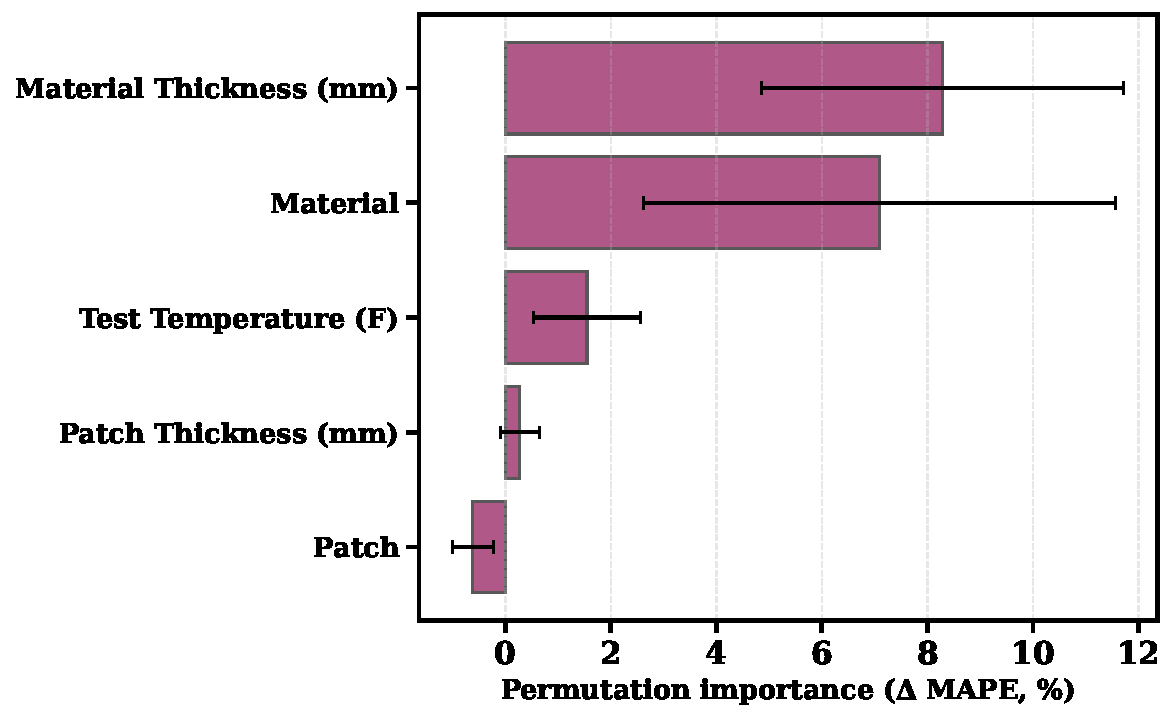
\includegraphics[width=\linewidth]{Figures/patched_feature_importance.pdf}
        \caption*{(a) Patched specimens.}
        \label{fig:feat_patched}
    \end{minipage}
    \hfill
    % Second image
    \begin{minipage}{0.45\textwidth}
        \centering
        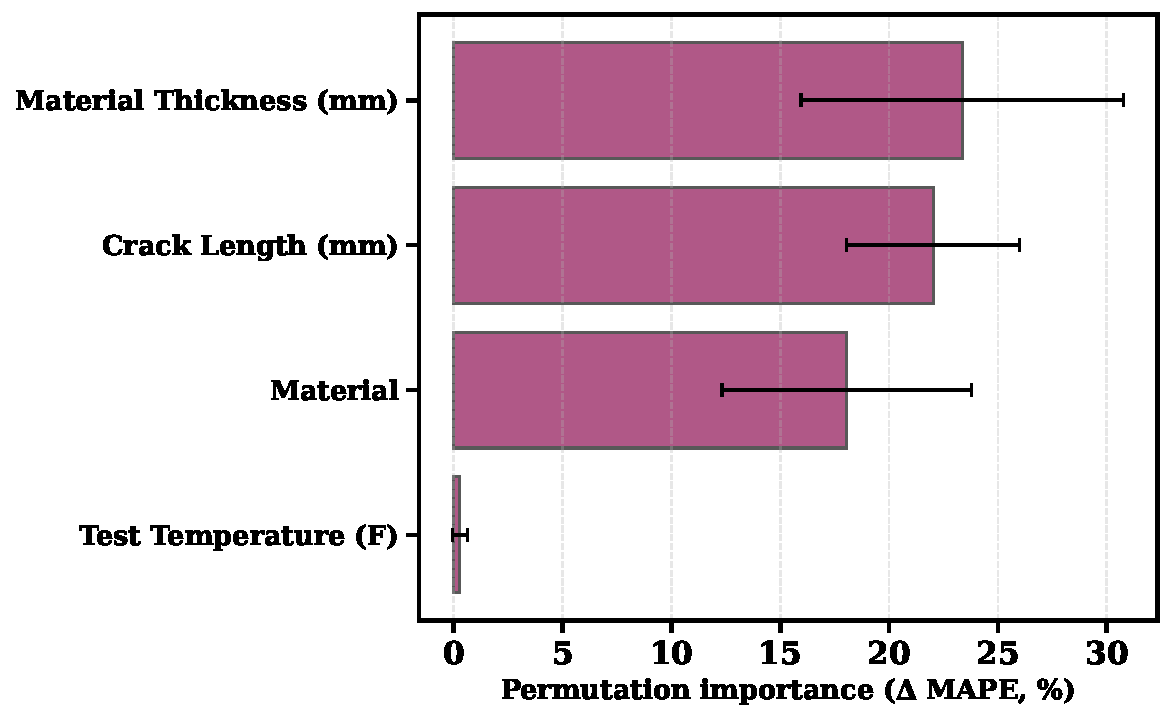
\includegraphics[width=\linewidth]{Figures/unpatched_feature_importance.pdf}
        \caption*{(b) Unpatched specimens.}
        \label{fig:feat_unpatched}
    \end{minipage}
    
    % Main caption for the whole figure
    \caption{Permutation feature importance in the original input space for the patched and unpatched dataset.}
    \label{fig:feature_importance}
\end{figure}

\subsection{Synthetic Data Generation}
\label{subsec:synthetic}
Because physical testing is costly and time-consuming, a \textit{Gaussian Mixture Model (GMM)} was used to oversample the cross-validation training folds. The GMM assumes that the data are drawn from a mixture of several Gaussian distributions and estimates the joint distribution of the inputs and the output, so that new, statistically representative samples can be drawn \cite{chokwitthaya2020applying}. In this study, the GMM used three mixture components with a full covariance structure, and each augmented training fold was enlarged to 300 samples.

To keep the synthetic data from biasing the evaluation, the leakage-free protocol in Section~\ref{sec:data-preprocessing} was applied as follows. Only the real samples (experimental, finite-element, and theoretical) were treated as ground truth. A 20\% stratified hold-out test set of real samples was reserved at the outset and never used for fitting, hyperparameter selection, augmentation, or preprocessing. The remaining real data formed the training pool and were split by 5-fold cross-validation; within each fold the GMM was fit on the training partition only and used to augment that partition, while the validation fold contained real data exclusively. The final regression-model performance was then reported on the untouched real hold-out test set. This separation ensures that no synthetic sample leaks across folds and prevents the optimistic bias that would otherwise arise.


The quality of the synthetic data was checked with the \textit{Kolmogorov–Smirnov (KS)} test, which compares the distribution of each generated feature with that of the original data \cite{an1933sulla}. The generation followed an acceptance protocol: the categorical inputs were sampled jointly with the numerical variables and decoded onto the existing classes only, the numerical values were clipped to the physical range observed in the baseline, and the near-discrete design inputs (such as the test temperature and the patch thickness) were snapped to their valid values. Sampling was repeated, up to five attempts, until every feature passed the KS test at the 5\% significance level. The accepted sets passed all KS tests (all $p>0.05$), with only a small difference in the correlation structure between the synthetic and the original data (0.13 for the patched and 0.15 for the unpatched dataset).
Figure~\ref{fig:synthetic_dist} overlays the baseline and synthetic distributions of the numerical variables for both datasets, together with the per-feature KS $p$-values. The close overlap between the two distributions confirms that the synthetic samples reproduce the marginal distributions of the real data while remaining within physically admissible ranges.

\begin{figure}[ht!]
\centering
\begin{minipage}{0.49\textwidth}
  \centering
  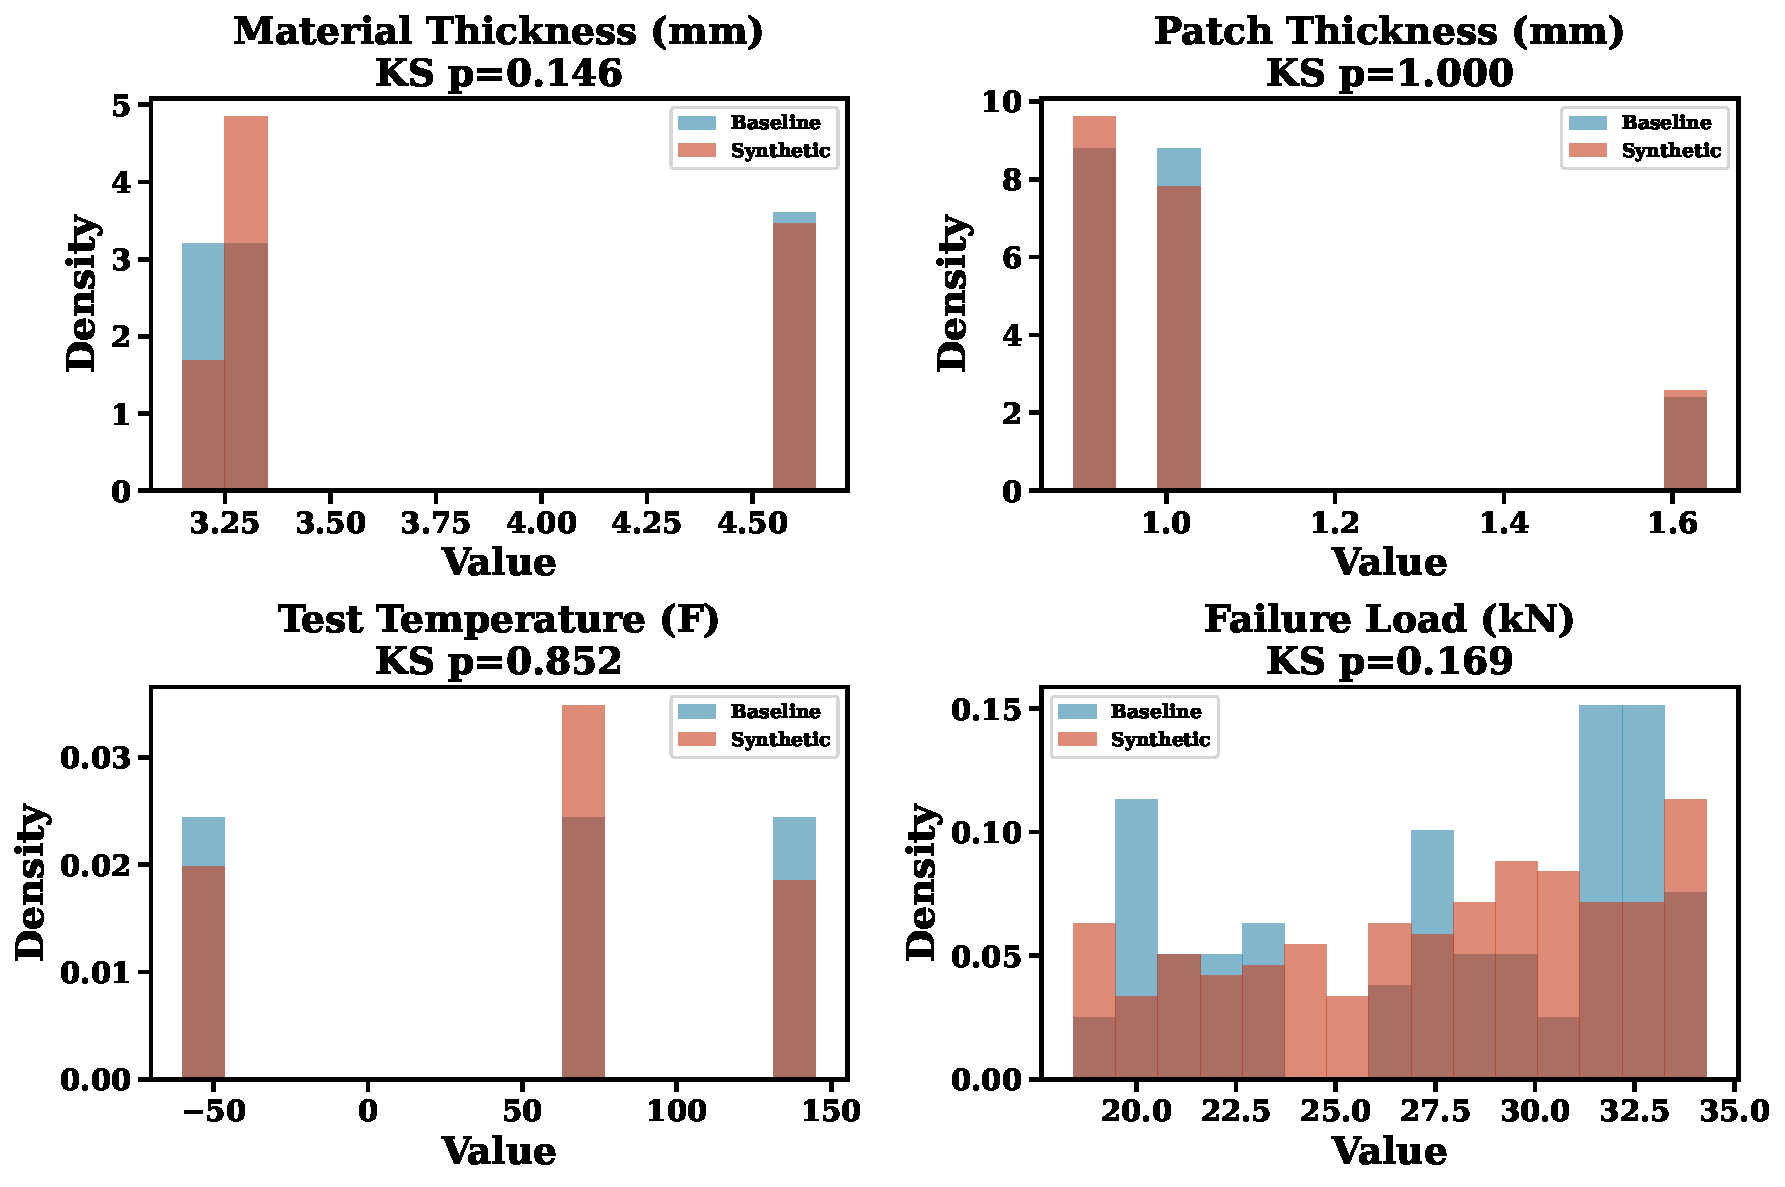
\includegraphics[width=\linewidth]{Figures/patched_synthetic_distributions.pdf}
  \caption*{(a) Patched dataset.}
\end{minipage}
\hfill
\begin{minipage}{0.49\textwidth}
  \centering
  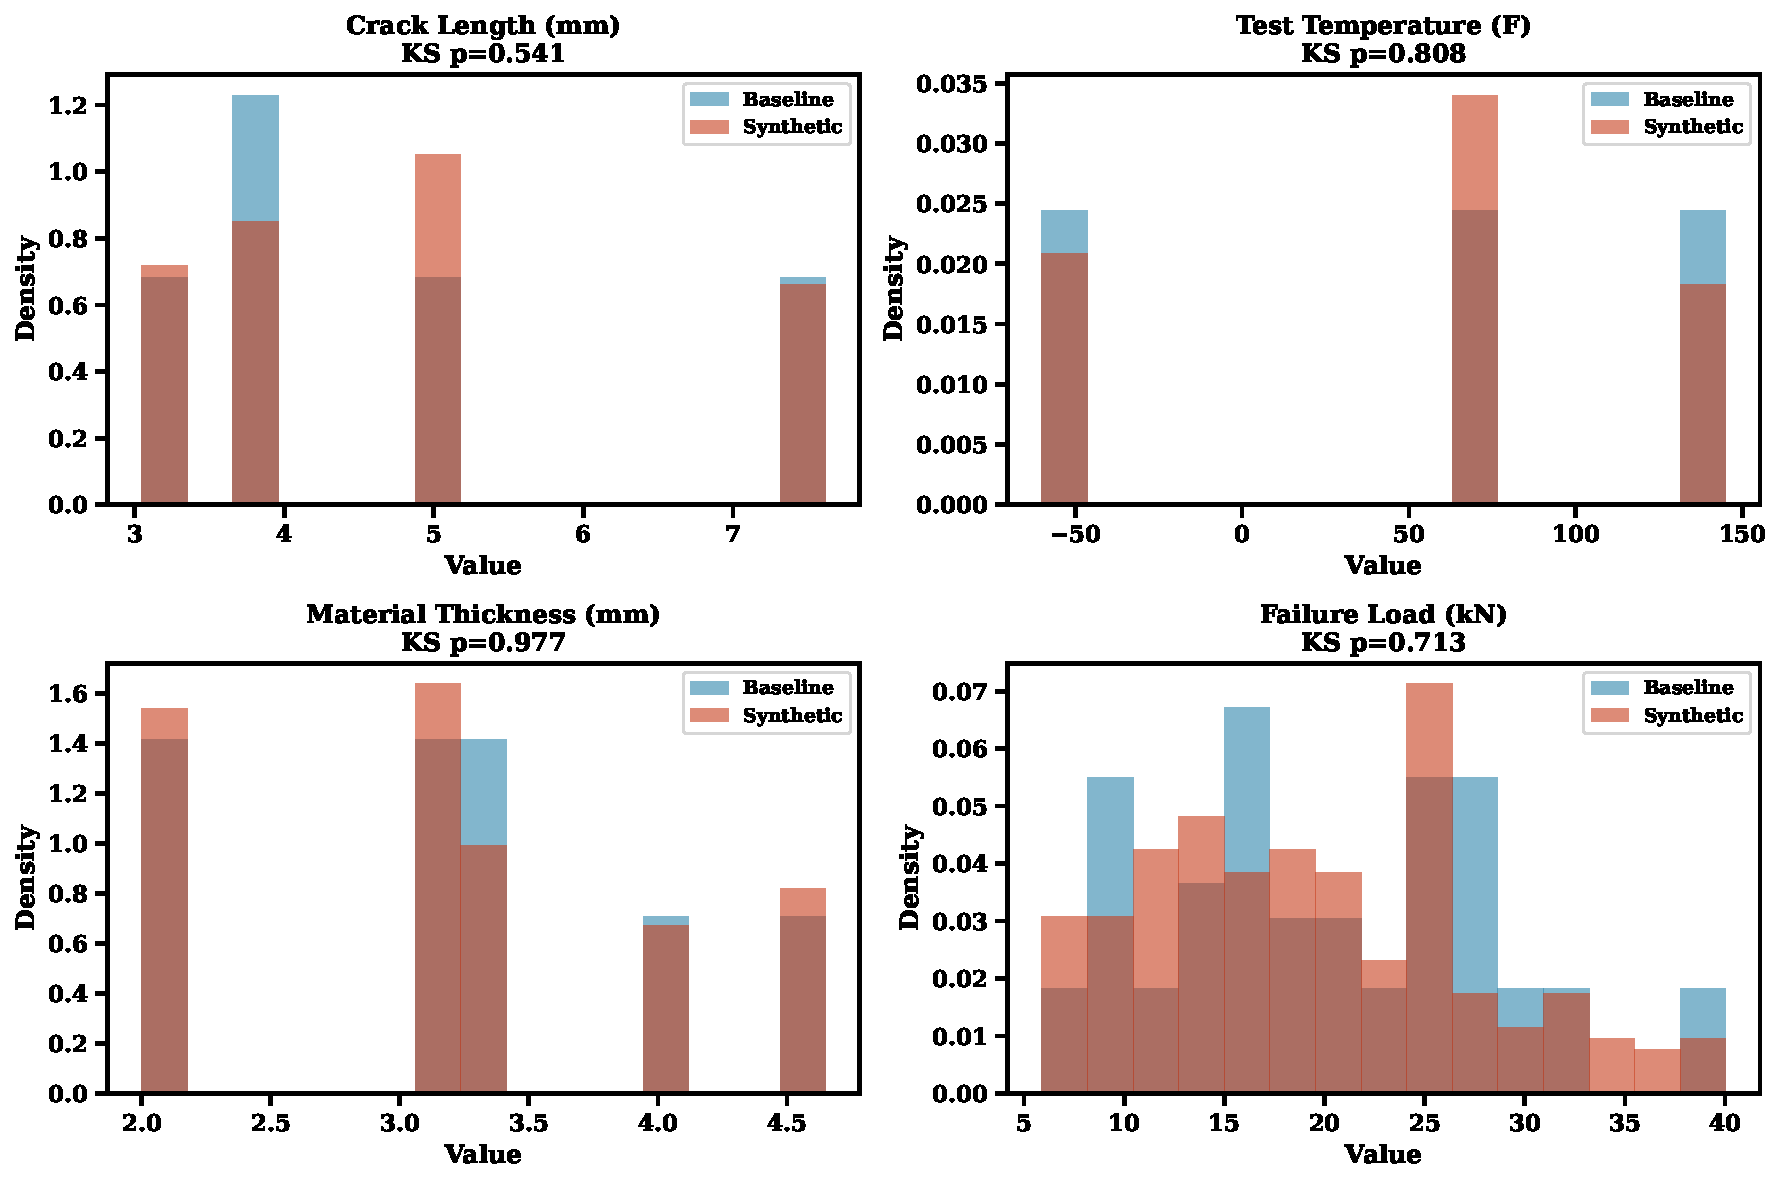
\includegraphics[width=\linewidth]{Figures/unpatched_synthetic_distributions.pdf}
  \caption*{(b) Unpatched dataset.}
\end{minipage}
\caption{Baseline versus GMM-generated synthetic distributions of the numerical variables, with the per-feature Kolmogorov--Smirnov $p$-values, for the (a) patched and (b) unpatched datasets.}
\label{fig:synthetic_dist}
\end{figure}

\subsection{Preprocessing}
Prior to training, the categorical inputs (\textit{Material} and \textit{Patch}) were transformed with one-hot encoding, so that each category is represented by a binary indicator vector and no artificial ordering is introduced among the classes. The numerical inputs were standardized with a standard scaler. To prevent information leakage, the scaler, the encoder, and the GMM generator were fit only on the training partition of each cross-validation fold \cite{schober2021statistics, pedregosa2011scikit}.For the final hold-out evaluation, the hold-out test set was transformed with a preprocessor fitted on the augmented training pool only and was never included in cross-validation or hyperparameter tuning.


\section{Results and Discussion}\label{sec:results-discussion}

The regression models were evaluated under the leakage-free protocol described in Section~\ref{sec:data-preprocessing}: hyperparameters were selected by 5-fold cross-validation on the real training pool, and final accuracy was reported on the untouched real hold-out test set. Table~\ref{tab:model_comparison}, the bar charts in Figures~\ref{fig:patched_bar_results} and~\ref{fig:unpatched_bar_results}, and the scatter plots in Figures~\ref{fig:patched_scatter_results} and~\ref{fig:unpatched_scatter_results} all report the same hold-out test metrics for the best configuration of each model. Cross-validated results for the full 116-configuration search space are provided separately in the appendix (Tables~\ref{tab:patched_allconfigs} and~\ref{tab:unpatched_allconfigs}).


\subsection{Patched Specimen Predictions}
On the real hold-out test set, Support Vector Regression (SVR) achieved the lowest error (MAPE 3.73\%, $R^2$ 0.937), followed closely by LightGBM (4.24\%, $R^2$ 0.919), KAN (4.59\%, $R^2$ 0.911), and Random Forest (4.64\%, $R^2$ 0.907). The selected ANN ([128, 64, 32, 16, 8], Leaky ReLU, learning rate 0.001, no dropout) reached a hold-out MAPE of 5.81\% and $R^2$ of 0.874, indicating that the ANN remains competitive although it was not the top performer on the patched dataset.

\begin{figure}[h!]
    \centering
    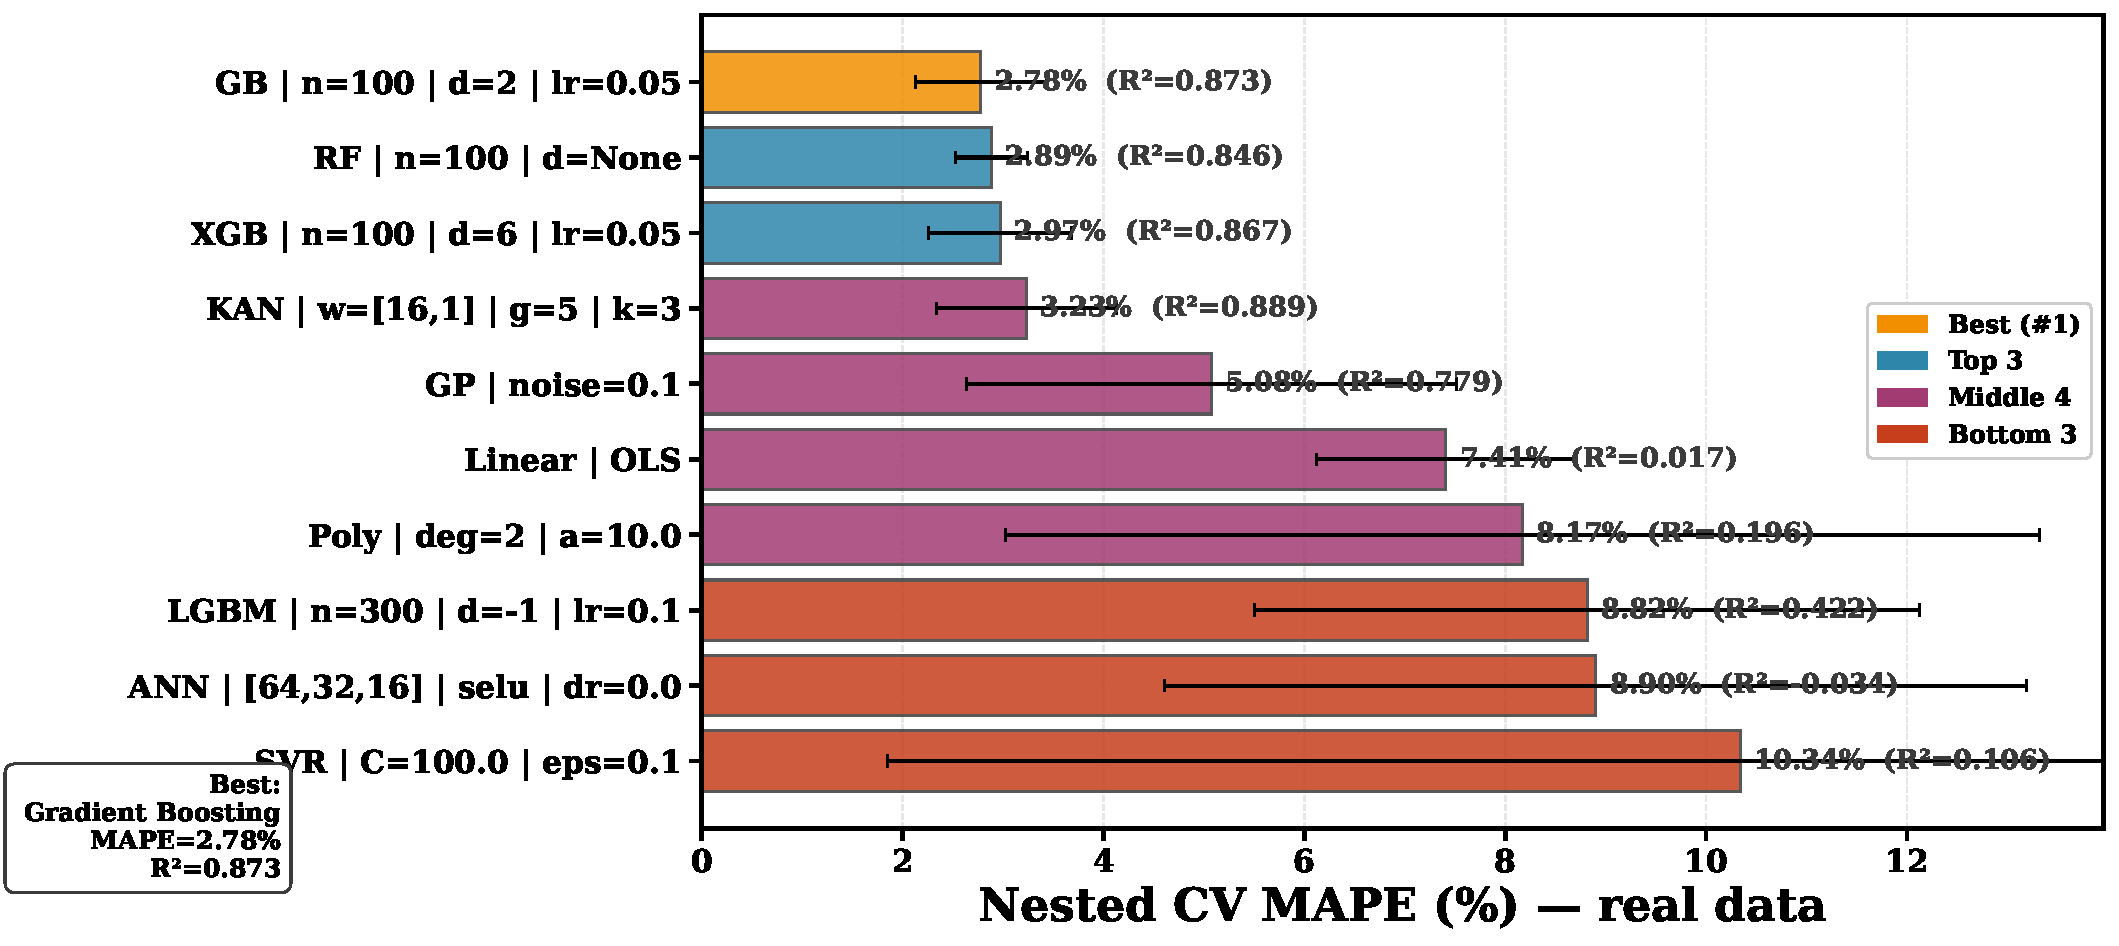
\includegraphics[width=0.85\linewidth]{Figures/patched_all_models_bar.pdf}
    \caption{Hold-out test MAPE for patched specimens: all ten regression models ranked by hold-out error (best configuration per model).}
    \label{fig:patched_bar_results}
\end{figure}

\begin{figure}[h!]
    \centering
    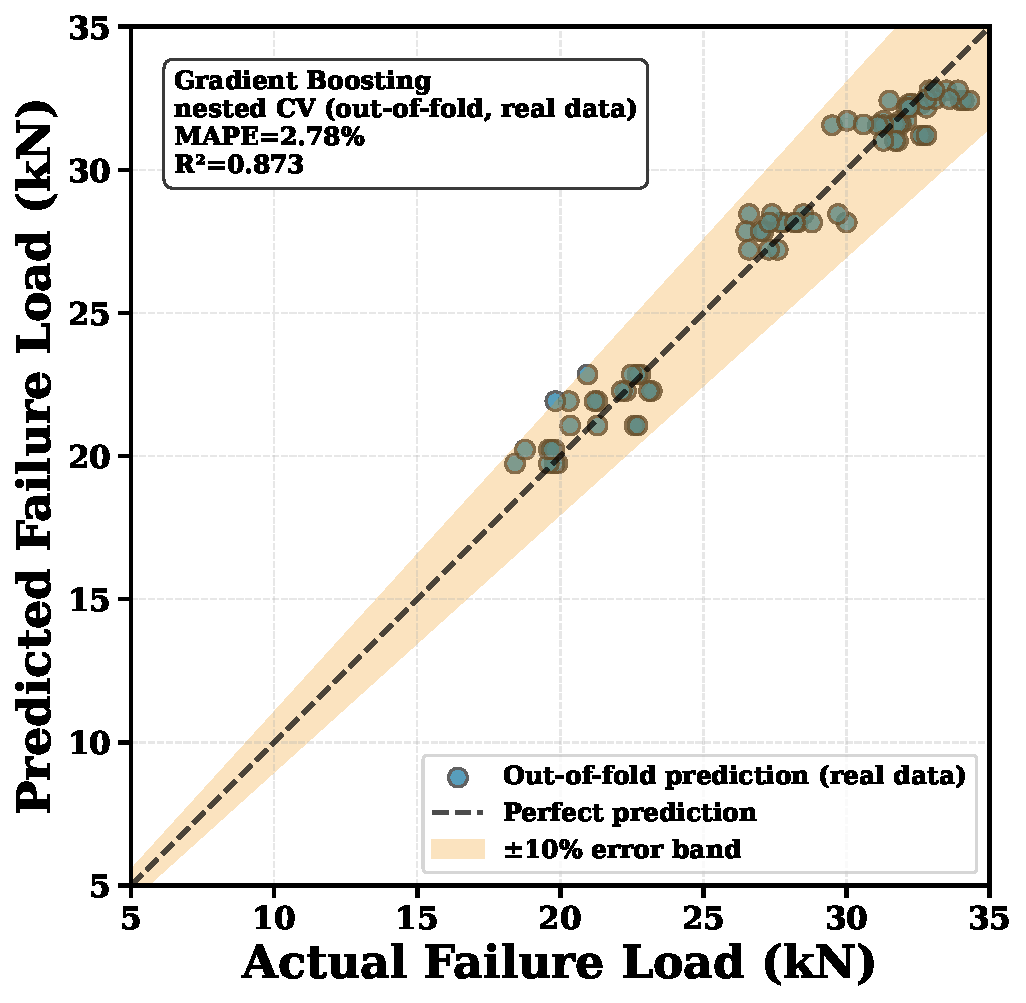
\includegraphics[width=0.65\linewidth]{Figures/patched_scatter.pdf}
    \caption{Hold-out test predictions of the best-performing model (Support Vector Regression) for patched specimens: actual versus predicted failure load (MAPE 3.73\%, $R^2 = 0.937$). The dashed line represents perfect prediction and the shaded region indicates a $\pm$10\% error band.}
    \label{fig:patched_scatter_results}
\end{figure}

Figure~\ref{fig:patched_bar_results} ranks the ten models by hold-out MAPE and confirms that Support Vector Regression is the most accurate, followed by LightGBM, KAN, and Random Forest, while linear regression shows the largest error. The hold-out scatter plot in Figure~\ref{fig:patched_scatter_results} shows that most real test points fall within the $\pm$10\% band for the same best model (SVR).



\subsection{Unpatched Specimen Predictions}

For the unpatched specimens, XGBoost delivered the best hold-out accuracy (MAPE 3.18\%, $R^2$ 0.994), with Gradient Boosting (4.48\%, $R^2$ 0.984) and Random Forest (4.56\%, $R^2$ 0.988) also performing strongly. The selected ANN ([64, 32, 16], SELU, learning rate 0.001, no dropout) attained a hold-out MAPE of 5.37\% and $R^2$ of 0.981. Although the unpatched ANN shows a higher $R^2$ than the patched ANN, this reflects the greater variance of the unpatched failure loads rather than a lower relative error.

\begin{figure}[ht]
    \centering
    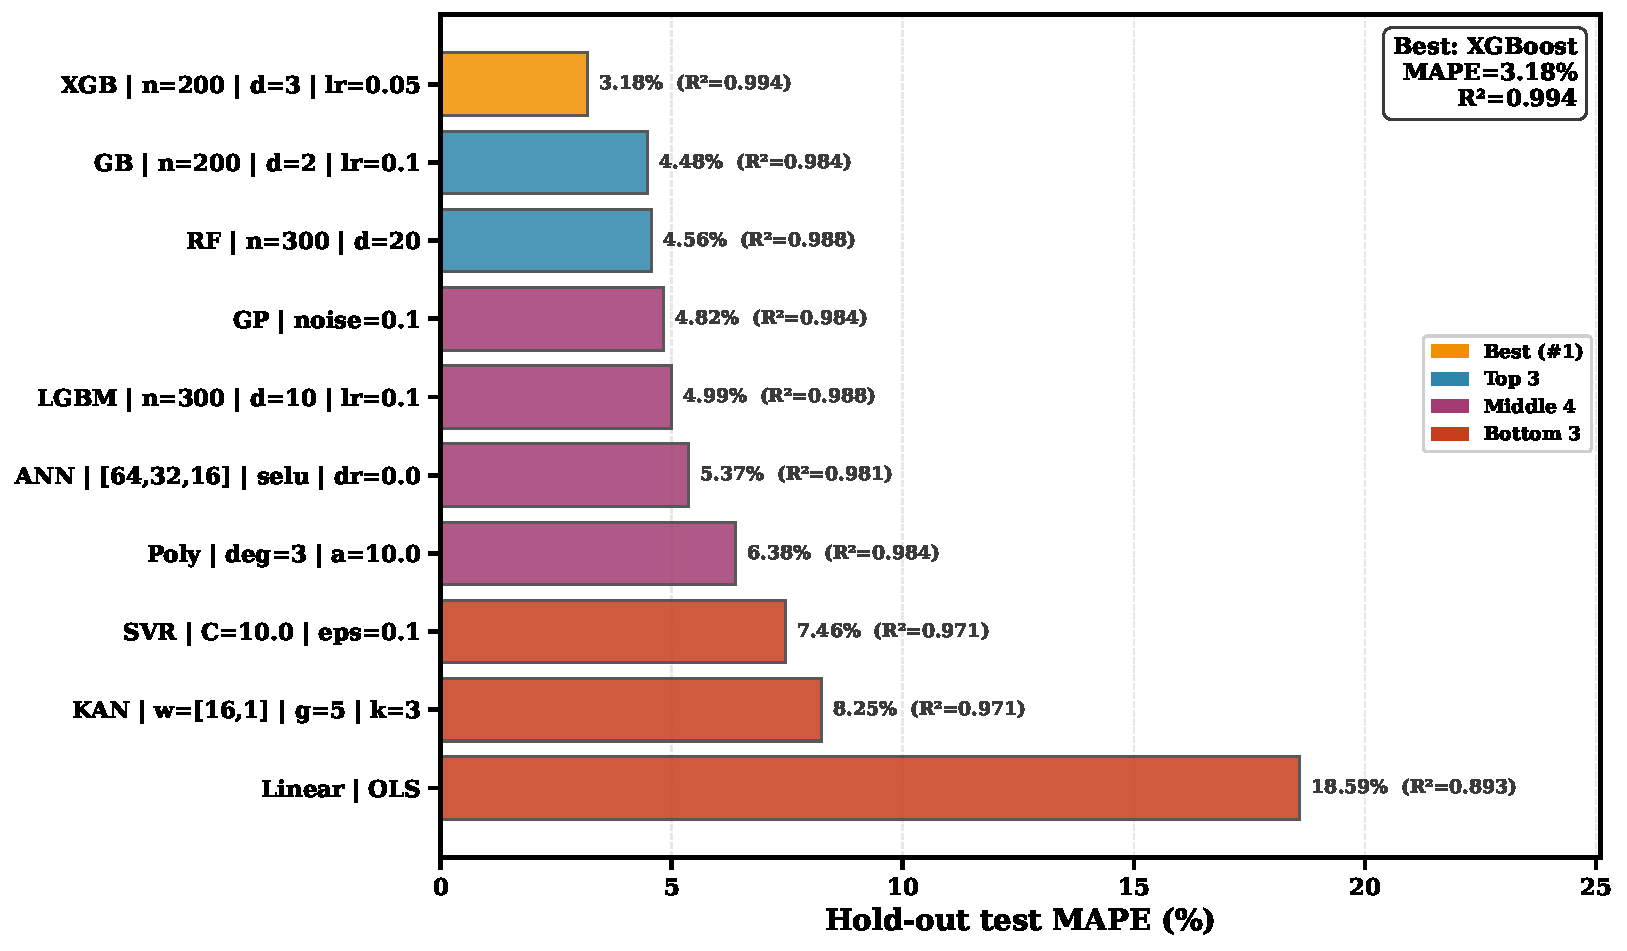
\includegraphics[width=0.85\linewidth]{Figures/unpatched_all_models_bar.pdf}
    \caption{Hold-out test MAPE for unpatched specimens: all ten regression models ranked by hold-out error (best configuration per model).}
    \label{fig:unpatched_bar_results}
\end{figure}

\begin{figure}[ht]
    \centering
    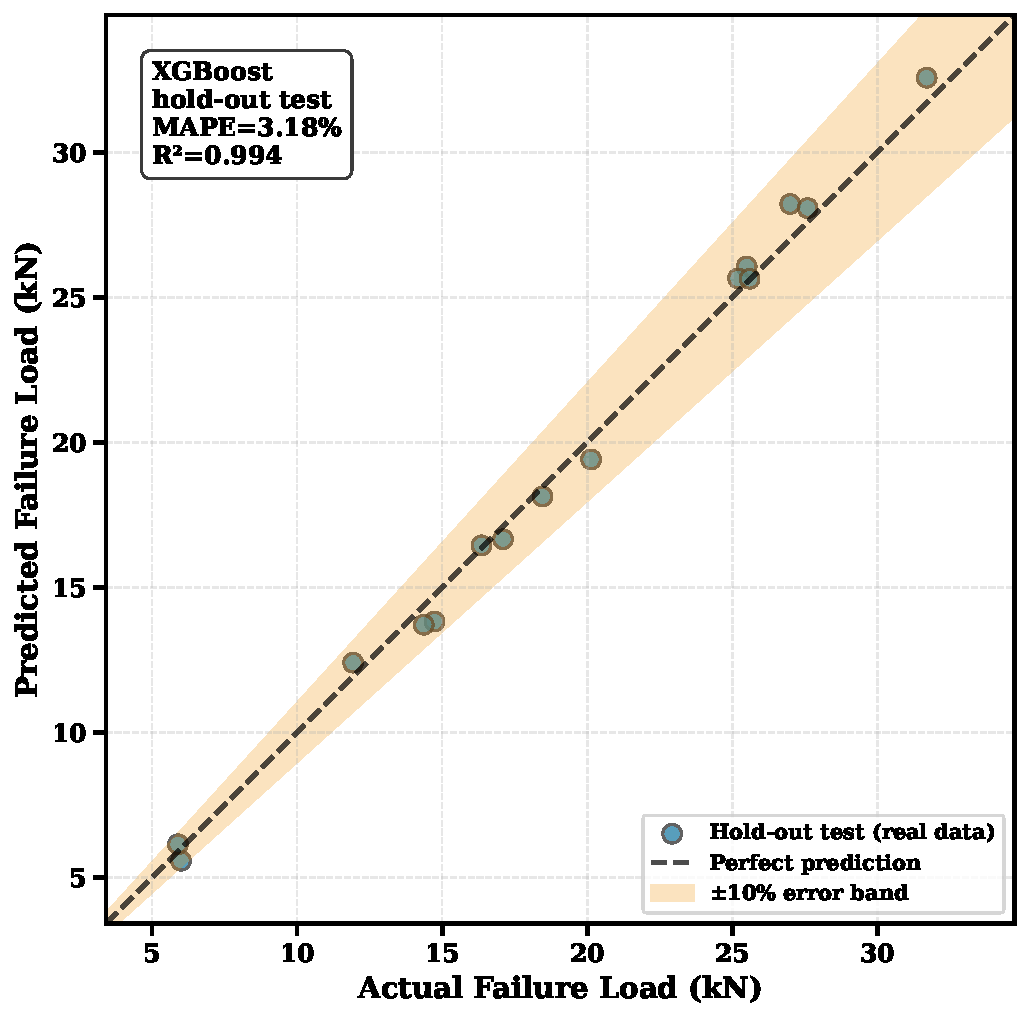
\includegraphics[width=0.65\linewidth]{Figures/unpatched_scatter.pdf}
    \caption{Hold-out test predictions of the best-performing model (XGBoost) for unpatched specimens: actual versus predicted failure load (MAPE 3.18\%, $R^2 = 0.994$). The dashed line represents perfect prediction and the shaded region indicates a $\pm$10\% error band.}
    \label{fig:unpatched_scatter_results}
\end{figure}

Figure~\ref{fig:unpatched_bar_results} shows that XGBoost achieved the lowest hold-out error, with the other tree-ensemble models also in the top group, whereas linear regression performed poorly. The hold-out scatter plot in Figure~\ref{fig:unpatched_scatter_results} shows a close agreement with the perfect-prediction line for the same best model (XGBoost), with most points within the $\pm$10\% band.

\subsection{Comparison and Practical Implications}

Table~\ref{tab:model_comparison} compares all regression models on the real hold-out test set (sorted by patched hold-out MAPE). For the patched specimens, classical and ensemble regressors (especially SVR and LightGBM) matched or exceeded the ANN, whereas for the unpatched specimens XGBoost and the other tree ensembles were the most accurate. The KAN, included as a state-of-the-art alternative, performed competitively on the patched dataset (4.59\% MAPE) but was less accurate on the unpatched case (8.25\% MAPE). Overall, the results indicate that the FE-augmented, leakage-free framework supports reliable failure-load prediction within the tested design space, while the optimal regressor depends on the dataset and no single model dominated both cases.



\begin{table}[ht]
    \centering
    \caption{Best regression model configuration with cross-validation and hold-out test performance for each dataset.}
    \label{tab:model_summary}
\begin{tabular}{@{}lcc@{}}
\toprule
\textbf{Parameter} & \textbf{Patched Dataset} & \textbf{Unpatched Dataset} \\
\midrule
Best model & Support Vector Regression & XGBoost \\ \hline
 Hyperparameters & \makecell{RBF kernel, $C=100$,\\$\varepsilon=0.5$ }& \makecell{200 trees, depth 3,\\ learning rate 0.05 }\\
\midrule
Baseline CV MAPE (\%) & 3.19 & 6.10 \\
Aug. CV MAPE (\%) & 4.68 $\pm$ 0.66 & 7.81 $\pm$ 2.59 \\
Baseline CV $R^2$ & 0.923 & 0.933 \\
Augmented CV $R^2$ & 0.816 $\pm$ 0.185 & 0.955 $\pm$ 0.021 \\
\midrule
Hold-out MAPE (\%) & 3.73 & 3.18 \\
Hold-out $R^2$ & 0.937 & 0.994 \\
\bottomrule
\end{tabular}
\end{table}

Table~\ref{tab:model_summary} summarizes the best-performing model for each dataset, including the cross-validated metrics used for hyperparameter selection (baseline CV on real data only, and augmented CV with GMM synthetic samples in the training folds) and the final hold-out test results. The patched top performer (SVR, 3.73\% hold-out MAPE) corresponds to an average absolute error of approximately 1.05~kN on a mean failure load of 28.22~kN, whereas the unpatched top performer (XGBoost, 3.18\% hold-out MAPE) corresponds to approximately 0.61~kN on a mean of 19.17~kN.



\begin{table}[H]
\centering
\caption{Comparison of regression models (mean absolute percentage error and $R^2$ on the real hold-out test set).}
\label{tab:model_comparison}
\begin{tabular}{lcccc}
\toprule
 & \multicolumn{2}{c}{\textbf{Patched}} & \multicolumn{2}{c}{\textbf{Unpatched}} \\
\textbf{Model} & \textbf{MAPE (\%)} & \textbf{$R^2$} & \textbf{MAPE (\%)} & \textbf{$R^2$} \\
\midrule
\textbf{Support Vector Regression} & \textbf{3.73} & \textbf{0.937} & 7.46  & 0.971 \\
LightGBM                  & 4.24 & 0.919 & 4.99  & 0.988 \\
KAN                       & 4.59 & 0.911 & 8.25  & 0.971 \\
Random Forest             & 4.64 & 0.907 & 4.56  & 0.988 \\
Gradient Boosting         & 5.21 & 0.882 & 4.48  & 0.984 \\
\textbf{XGBoost}            & 5.23 & 0.880 & \textbf{3.18}  & \textbf{0.994} \\
ANN (this study)          & 5.81 & 0.874 & 5.37  & 0.981 \\
Polynomial Regression     & 6.11 & 0.850 & 6.38  & 0.984 \\
Gaussian Process          & 6.28 & 0.849 & 4.82  & 0.984 \\
Linear Regression         & 8.28 & 0.727 & 18.59 & 0.893 \\
\bottomrule
\end{tabular}
\end{table}





\section{Conclusions}\label{sec:conclusion}

The experimental results showed that bonded composite patch repairs effectively improved the load-carrying capacity of both Al 6061 and A36 steel specimens under room and low-temperature conditions. Although the effectiveness of the repairs decreased at elevated temperature because of adhesive softening, both glass-fiber and carbon-fiber patches continued to provide comparable improvements over the unpatched specimens, indicating that patch type had no significant effect on repair effectiveness at elevated temperature and that both patch types can be considered equally reliable choices in this condition. In addition, increasing the patch thickness further enhanced the repair performance, highlighting the beneficial effect of patch thickness on repair effectiveness.

To complement the experimental investigation, machine-learning regression models were developed to predict the static failure loads ($P_{\mathrm{cr}}$) of unpatched specimens and specimens repaired with glass- or carbon-fiber composite patches under varying temperature conditions.  Although the available experimental dataset was limited, the combined use of theoretical calculations, finite element (FE) predictions, and GMM-generated synthetic data enabled the regression models to learn the underlying temperature-dependent behavior with an acceptable accuracy. 


Under the leakage-free evaluation protocol, the best hold-out regression models achieved MAPE values of 3.73\% (Support Vector Regression, patched specimens) and 3.18\% (XGBoost, unpatched specimens), with $R^2$ values of 0.937 and 0.994, respectively. The regression models demonstrated good generalization capability, with hold-out $R^2$ values greater than 0.87 for all approaches except linear regression, and hyperparameters were selected by cross-validation on real training data augmented with GMM synthetic samples. These findings indicate the potential of machine-learning regression models for predicting static failure loads within the tested design space, highlight the benefits of synthetic data augmentation when experimental data are limited, and suggest that broader validation on additional materials, temperatures, and patch configurations remains necessary before general predictive reliability can be claimed. The developed regression models are applicable within the range of parameters investigated in this study, including Al 6061 and A36 steel substrates, temperatures from -60$^\circ$F to 145$^\circ$F, substrate thicknesses of 1/8 inch (3.18 mm) and 0.190 inches (4.83 mm), and patch thicknesses between 1.0 mm and 1.64 mm. Overall, the proposed FE-augmented machine-learning framework demonstrates the potential of combining experimental data, finite element analysis, and regression-based predictive modelling to efficiently predict the static performance of bonded composite patch repairs while reducing the need for extensive experimental testing.

\FloatBarrier
\newpage
\section*{References}
%\bibliographystyle{MDPI}
\bibliography{reference.bib}
\newpage
\section*{Appendix}
The tables below list 5-fold cross-validated MAPE and $R^2$ for all 116 hyperparameter configurations per dataset (augmented training folds). These cross-validation values differ from the bar charts, scatter plots, and comparison tables in the main text, which report hold-out test metrics on untouched real data only; the ranking of configurations may therefore differ between the appendix and the main-text figures.


\begin{center}
\footnotesize
\begin{longtable}{@{}p{8.2cm} c c@{}}
\caption{Full cross-validation results for every configuration evaluated (patched dataset). Values are augmented 5-fold CV metrics used for hyperparameter selection, not hold-out test results.} \label{tab:patched_allconfigs} \\
\toprule
\textbf{Configuration} & \textbf{CV MAPE (\%)} & \textbf{CV $R^2$} \\
\midrule
\endfirsthead
\multicolumn{3}{c}{\tablename\ \thetable\ -- Continued from previous page} \\
\toprule
\textbf{Configuration} & \textbf{CV MAPE (\%)} & \textbf{CV $R^2$} \\
\midrule
\endhead
\midrule \multicolumn{3}{r}{Continued on next page} \\
\endfoot
\bottomrule
\endlastfoot
\multicolumn{3}{@{}l}{\textbf{Linear Regression}} \\
\quad None (OLS) & 6.69 $\pm$ 0.88 & 0.703 \\
\midrule
\multicolumn{3}{@{}l}{\textbf{Polynomial Regression}} \\
\quad degree 3, $\alpha$=10 & 4.86 $\pm$ 0.89 & 0.821 \\
\quad degree 2, $\alpha$=1 & 4.93 $\pm$ 0.72 & 0.828 \\
\quad degree 3, $\alpha$=1 & 4.96 $\pm$ 1.35 & 0.800 \\
\quad degree 2, $\alpha$=0.1 & 4.98 $\pm$ 0.82 & 0.828 \\
\quad degree 3, $\alpha$=0.1 & 5.09 $\pm$ 1.72 & 0.768 \\
\quad degree 2, $\alpha$=10 & 5.36 $\pm$ 1.15 & 0.820 \\
\midrule
\multicolumn{3}{@{}l}{\textbf{Support Vector Regression}} \\
\quad RBF kernel, $C$=100, $\varepsilon$=0.5 & 4.68 $\pm$ 0.66 & 0.816 \\
\quad RBF kernel, $C$=10, $\varepsilon$=0.1 & 4.74 $\pm$ 0.73 & 0.833 \\
\quad RBF kernel, $C$=100, $\varepsilon$=0.1 & 4.75 $\pm$ 0.79 & 0.790 \\
\quad RBF kernel, $C$=10, $\varepsilon$=0.5 & 4.98 $\pm$ 0.73 & 0.814 \\
\quad RBF kernel, $C$=1, $\varepsilon$=0.1 & 7.06 $\pm$ 2.36 & 0.767 \\
\quad RBF kernel, $C$=1, $\varepsilon$=0.5 & 7.25 $\pm$ 2.35 & 0.758 \\
\midrule
\multicolumn{3}{@{}l}{\textbf{Random Forest}} \\
\quad 300 trees, depth 10, min.\ split 5 & 4.70 $\pm$ 0.86 & 0.837 \\
\quad 300 trees, depth 20, min.\ split 5 & 4.70 $\pm$ 0.86 & 0.837 \\
\quad 300 trees, depth None, min.\ split 5 & 4.70 $\pm$ 0.86 & 0.837 \\
\quad 200 trees, depth 10, min.\ split 5 & 4.70 $\pm$ 0.83 & 0.838 \\
\quad 200 trees, depth None, min.\ split 5 & 4.70 $\pm$ 0.83 & 0.838 \\
\quad 200 trees, depth 20, min.\ split 5 & 4.70 $\pm$ 0.83 & 0.838 \\
\quad 100 trees, depth 10, min.\ split 5 & 4.73 $\pm$ 0.83 & 0.841 \\
\quad 100 trees, depth 20, min.\ split 5 & 4.73 $\pm$ 0.83 & 0.841 \\
\quad 100 trees, depth None, min.\ split 5 & 4.73 $\pm$ 0.83 & 0.841 \\
\quad 100 trees, depth None, min.\ split 2 & 4.77 $\pm$ 0.87 & 0.840 \\
\quad 100 trees, depth 20, min.\ split 2 & 4.77 $\pm$ 0.87 & 0.840 \\
\quad 100 trees, depth 10, min.\ split 2 & 4.77 $\pm$ 0.87 & 0.840 \\
\quad 300 trees, depth 20, min.\ split 2 & 4.78 $\pm$ 0.86 & 0.835 \\
\quad 300 trees, depth None, min.\ split 2 & 4.78 $\pm$ 0.86 & 0.835 \\
\quad 300 trees, depth 10, min.\ split 2 & 4.78 $\pm$ 0.86 & 0.835 \\
\quad 200 trees, depth 20, min.\ split 2 & 4.78 $\pm$ 0.84 & 0.835 \\
\quad 200 trees, depth 10, min.\ split 2 & 4.78 $\pm$ 0.84 & 0.835 \\
\quad 200 trees, depth None, min.\ split 2 & 4.78 $\pm$ 0.84 & 0.835 \\
\midrule
\multicolumn{3}{@{}l}{\textbf{Gradient Boosting}} \\
\quad 100 trees, depth 3, lr 0.05 & 4.52 $\pm$ 1.10 & 0.845 \\
\quad 200 trees, depth 3, lr 0.05 & 4.69 $\pm$ 0.92 & 0.840 \\
\quad 100 trees, depth 3, lr 0.1 & 4.69 $\pm$ 0.88 & 0.842 \\
\quad 200 trees, depth 3, lr 0.1 & 4.78 $\pm$ 0.84 & 0.834 \\
\quad 200 trees, depth 2, lr 0.1 & 4.81 $\pm$ 0.84 & 0.846 \\
\quad 100 trees, depth 2, lr 0.1 & 4.82 $\pm$ 0.99 & 0.846 \\
\quad 200 trees, depth 2, lr 0.05 & 4.94 $\pm$ 0.98 & 0.843 \\
\quad 100 trees, depth 2, lr 0.05 & 5.08 $\pm$ 1.35 & 0.829 \\
\midrule
\multicolumn{3}{@{}l}{\textbf{XGBoost}} \\
\quad 100 trees, depth 3, lr 0.05 & 4.51 $\pm$ 1.19 & 0.845 \\
\quad 100 trees, depth 3, lr 0.1 & 4.55 $\pm$ 0.97 & 0.842 \\
\quad 200 trees, depth 3, lr 0.05 & 4.57 $\pm$ 1.00 & 0.838 \\
\quad 300 trees, depth 3, lr 0.05 & 4.68 $\pm$ 0.84 & 0.837 \\
\quad 100 trees, depth 6, lr 0.05 & 4.70 $\pm$ 0.97 & 0.834 \\
\quad 200 trees, depth 3, lr 0.1 & 4.73 $\pm$ 0.82 & 0.835 \\
\quad 300 trees, depth 3, lr 0.1 & 4.80 $\pm$ 0.81 & 0.833 \\
\quad 200 trees, depth 6, lr 0.05 & 4.87 $\pm$ 0.83 & 0.830 \\
\quad 100 trees, depth 6, lr 0.1 & 4.87 $\pm$ 0.83 & 0.829 \\
\quad 300 trees, depth 6, lr 0.05 & 4.87 $\pm$ 0.82 & 0.829 \\
\quad 300 trees, depth 6, lr 0.1 & 4.87 $\pm$ 0.82 & 0.829 \\
\quad 200 trees, depth 6, lr 0.1 & 4.87 $\pm$ 0.82 & 0.829 \\
\midrule
\multicolumn{3}{@{}l}{\textbf{LightGBM}} \\
\quad 300 trees, depth -1, lr 0.1 & 4.38 $\pm$ 0.84 & 0.840 \\
\quad 300 trees, depth 10, lr 0.1 & 4.38 $\pm$ 0.84 & 0.840 \\
\quad 300 trees, depth 10, lr 0.05 & 4.44 $\pm$ 0.78 & 0.845 \\
\quad 300 trees, depth -1, lr 0.05 & 4.44 $\pm$ 0.78 & 0.845 \\
\quad 200 trees, depth 10, lr 0.1 & 4.45 $\pm$ 0.79 & 0.843 \\
\quad 200 trees, depth -1, lr 0.1 & 4.45 $\pm$ 0.79 & 0.843 \\
\quad 200 trees, depth -1, lr 0.05 & 4.46 $\pm$ 0.73 & 0.848 \\
\quad 200 trees, depth 10, lr 0.05 & 4.46 $\pm$ 0.73 & 0.848 \\
\quad 100 trees, depth -1, lr 0.1 & 4.51 $\pm$ 0.72 & 0.846 \\
\quad 100 trees, depth 10, lr 0.1 & 4.51 $\pm$ 0.72 & 0.846 \\
\quad 100 trees, depth -1, lr 0.05 & 4.76 $\pm$ 0.78 & 0.844 \\
\quad 100 trees, depth 10, lr 0.05 & 4.76 $\pm$ 0.78 & 0.844 \\
\midrule
\multicolumn{3}{@{}l}{\textbf{Gaussian Process}} \\
\quad RBF+white kernel, noise 0.1 & 5.21 $\pm$ 0.83 & 0.827 \\
\quad RBF+white kernel, noise 1 & 5.21 $\pm$ 0.83 & 0.827 \\
\midrule
\multicolumn{3}{@{}l}{\textbf{KAN}} \\
\quad width [16, 1], grid 5, order 3, lr 0.01 & 4.92 $\pm$ 0.92 & 0.831 \\
\midrule
\multicolumn{3}{@{}l}{\textbf{ANN (this study)}} \\
\quad [128, 64, 32, 16, 8], Leaky ReLU, lr 0.001, dropout 0 & 5.03 $\pm$ 0.57 & 0.822 \\
\quad [128, 64, 32, 16, 8], SELU, lr 0.001, dropout 0 & 5.17 $\pm$ 0.30 & 0.822 \\
\quad [128, 64, 32, 16, 8], ReLU, lr 0.001, dropout 0 & 5.18 $\pm$ 0.61 & 0.809 \\
\quad [128, 64, 32, 16, 8], ELU, lr 0.001, dropout 0 & 5.25 $\pm$ 0.31 & 0.822 \\
\quad [128, 64, 32], Leaky ReLU, lr 0.001, dropout 0 & 5.26 $\pm$ 1.10 & 0.817 \\
\quad [128, 64, 32], SELU, lr 0.001, dropout 0 & 5.32 $\pm$ 0.72 & 0.817 \\
\quad [128, 64, 32], ReLU, lr 0.001, dropout 0 & 5.34 $\pm$ 1.16 & 0.817 \\
\quad [128, 64, 32], ELU, lr 0.001, dropout 0 & 5.39 $\pm$ 0.61 & 0.808 \\
\quad [128, 64, 32], SELU, lr 0.001, dropout 0.1 & 5.41 $\pm$ 1.14 & 0.796 \\
\quad [32, 16, 8], SELU, lr 0.001, dropout 0 & 5.45 $\pm$ 1.02 & 0.785 \\
\quad [64, 32, 16], Leaky ReLU, lr 0.001, dropout 0 & 5.45 $\pm$ 1.20 & 0.814 \\
\quad [64, 32, 16], ReLU, lr 0.001, dropout 0 & 5.50 $\pm$ 0.95 & 0.799 \\
\quad [64, 32, 16], SELU, lr 0.001, dropout 0 & 5.61 $\pm$ 0.97 & 0.789 \\
\quad [64, 32, 16], SELU, lr 0.001, dropout 0.1 & 5.63 $\pm$ 0.95 & 0.782 \\
\quad [64, 32, 16, 8], ReLU, lr 0.001, dropout 0 & 5.63 $\pm$ 0.71 & 0.796 \\
\quad [128, 64, 32], ReLU, lr 0.001, dropout 0.1 & 5.65 $\pm$ 1.28 & 0.812 \\
\quad [64, 32, 16], ELU, lr 0.001, dropout 0 & 5.70 $\pm$ 0.80 & 0.782 \\
\quad [64, 32, 16, 8], SELU, lr 0.001, dropout 0 & 5.72 $\pm$ 1.02 & 0.772 \\
\quad [128, 64, 32], ELU, lr 0.001, dropout 0.1 & 5.73 $\pm$ 1.22 & 0.781 \\
\quad [32, 16, 8], Leaky ReLU, lr 0.001, dropout 0 & 5.78 $\pm$ 0.82 & 0.779 \\
\quad [64, 32, 16], ELU, lr 0.001, dropout 0.1 & 5.80 $\pm$ 0.73 & 0.779 \\
\quad [64, 32, 16, 8], SELU, lr 0.001, dropout 0.1 & 5.86 $\pm$ 0.83 & 0.771 \\
\quad [128, 64, 32], Leaky ReLU, lr 0.001, dropout 0.1 & 5.89 $\pm$ 0.89 & 0.810 \\
\quad [32, 16, 8], ELU, lr 0.001, dropout 0 & 5.90 $\pm$ 1.15 & 0.753 \\
\quad [64, 32, 16, 8], Leaky ReLU, lr 0.001, dropout 0 & 5.91 $\pm$ 1.07 & 0.747 \\
\quad [64, 32, 16, 8], ELU, lr 0.001, dropout 0 & 5.96 $\pm$ 0.91 & 0.760 \\
\quad [32, 16, 8], ReLU, lr 0.001, dropout 0 & 5.99 $\pm$ 1.28 & 0.796 \\
\quad [128, 64, 32, 16, 8], SELU, lr 0.001, dropout 0.1 & 6.04 $\pm$ 1.41 & 0.780 \\
\quad [128, 64, 32, 16, 8], ELU, lr 0.001, dropout 0.1 & 6.17 $\pm$ 1.32 & 0.758 \\
\quad [128, 64, 32, 16, 8], ReLU, lr 0.001, dropout 0.1 & 6.20 $\pm$ 0.92 & 0.775 \\
\quad [32, 16, 8], Leaky ReLU, lr 0.001, dropout 0.1 & 6.22 $\pm$ 0.84 & 0.752 \\
\quad [64, 32, 16, 8], ELU, lr 0.001, dropout 0.1 & 6.22 $\pm$ 0.51 & 0.754 \\
\quad [32, 16, 8], SELU, lr 0.001, dropout 0.1 & 6.24 $\pm$ 1.14 & 0.750 \\
\quad [32, 16, 8], ELU, lr 0.001, dropout 0.1 & 6.52 $\pm$ 0.98 & 0.731 \\
\quad [32, 16, 8], ReLU, lr 0.001, dropout 0.1 & 6.74 $\pm$ 1.14 & 0.709 \\
\quad [64, 32, 16], ReLU, lr 0.001, dropout 0.1 & 7.01 $\pm$ 1.07 & 0.712 \\
\quad [64, 32, 16, 8], ReLU, lr 0.001, dropout 0.1 & 7.14 $\pm$ 1.40 & 0.632 \\
\quad [64, 32, 16], Leaky ReLU, lr 0.001, dropout 0.1 & 7.16 $\pm$ 1.31 & 0.732 \\
\quad [128, 64, 32, 16, 8], Leaky ReLU, lr 0.001, dropout 0.1 & 7.44 $\pm$ 0.60 & 0.652 \\
\quad [64, 32, 16, 8], Leaky ReLU, lr 0.001, dropout 0.1 & 7.68 $\pm$ 1.16 & 0.656 \\
\quad [128, 64, 32], tanh, lr 0.001, dropout 0.1 & 13.01 $\pm$ 7.77 & 0.003 \\
\quad [128, 64, 32], tanh, lr 0.001, dropout 0 & 15.24 $\pm$ 7.40 & -0.163 \\
\quad [32, 16, 8], tanh, lr 0.001, dropout 0.1 & 17.86 $\pm$ 3.88 & -0.385 \\
\quad [64, 32, 16, 8], tanh, lr 0.001, dropout 0.1 & 17.87 $\pm$ 3.86 & -0.388 \\
\quad [128, 64, 32, 16, 8], tanh, lr 0.001, dropout 0.1 & 17.88 $\pm$ 3.87 & -0.385 \\
\quad [64, 32, 16, 8], tanh, lr 0.001, dropout 0 & 17.92 $\pm$ 3.95 & -0.376 \\
\quad [32, 16, 8], tanh, lr 0.001, dropout 0 & 17.92 $\pm$ 3.97 & -0.375 \\
\quad [128, 64, 32, 16, 8], tanh, lr 0.001, dropout 0 & 17.93 $\pm$ 3.98 & -0.373 \\
\quad [64, 32, 16], tanh, lr 0.001, dropout 0.1 & 17.99 $\pm$ 4.29 & -0.354 \\
\quad [64, 32, 16], tanh, lr 0.001, dropout 0 & 18.01 $\pm$ 4.41 & -0.352 \\
\midrule
\end{longtable}
\end{center}
\newpage
\begin{center}
\footnotesize
\begin{longtable}{@{}p{8.2cm} c c@{}}
\caption{Full cross-validation results for every configuration evaluated (unpatched dataset). Values are augmented 5-fold CV metrics used for hyperparameter selection, not hold-out test results.} \label{tab:unpatched_allconfigs} \\
\toprule
\textbf{Configuration} & \textbf{CV MAPE (\%)} & \textbf{CV $R^2$} \\
\midrule
\endfirsthead
\multicolumn{3}{c}{\tablename\ \thetable\ -- Continued from previous page} \\
\toprule
\textbf{Configuration} & \textbf{CV MAPE (\%)} & \textbf{CV $R^2$} \\
\midrule
\endhead
\midrule \multicolumn{3}{r}{Continued on next page} \\
\endfoot
\bottomrule
\endlastfoot
\multicolumn{3}{@{}l}{\textbf{Linear Regression}} \\
\quad None (OLS) & 9.30 $\pm$ 4.35 & 0.912 \\
\midrule
\multicolumn{3}{@{}l}{\textbf{Polynomial Regression}} \\
\quad degree 3, $\alpha$=10 & 5.94 $\pm$ 2.38 & 0.965 \\
\quad degree 2, $\alpha$=1 & 6.22 $\pm$ 2.89 & 0.964 \\
\quad degree 2, $\alpha$=0.1 & 6.27 $\pm$ 2.95 & 0.964 \\
\quad degree 2, $\alpha$=10 & 6.37 $\pm$ 2.48 & 0.959 \\
\quad degree 3, $\alpha$=1 & 7.74 $\pm$ 5.87 & 0.941 \\
\quad degree 3, $\alpha$=0.1 & 8.26 $\pm$ 6.48 & 0.932 \\
\midrule
\multicolumn{3}{@{}l}{\textbf{Support Vector Regression}} \\
\quad RBF kernel, $C$=10, $\varepsilon$=0.1 & 8.74 $\pm$ 2.68 & 0.932 \\
\quad RBF kernel, $C$=10, $\varepsilon$=0.5 & 9.02 $\pm$ 2.70 & 0.930 \\
\quad RBF kernel, $C$=100, $\varepsilon$=0.1 & 9.08 $\pm$ 2.86 & 0.915 \\
\quad RBF kernel, $C$=100, $\varepsilon$=0.5 & 9.29 $\pm$ 3.43 & 0.915 \\
\quad RBF kernel, $C$=1, $\varepsilon$=0.5 & 12.48 $\pm$ 6.56 & 0.842 \\
\quad RBF kernel, $C$=1, $\varepsilon$=0.1 & 12.80 $\pm$ 7.20 & 0.839 \\
\midrule
\multicolumn{3}{@{}l}{\textbf{Random Forest}} \\
\quad 300 trees, depth None, min.\ split 5 & 9.91 $\pm$ 6.05 & 0.908 \\
\quad 300 trees, depth 20, min.\ split 5 & 9.91 $\pm$ 6.05 & 0.908 \\
\quad 300 trees, depth 10, min.\ split 5 & 9.91 $\pm$ 6.05 & 0.908 \\
\quad 200 trees, depth None, min.\ split 5 & 10.00 $\pm$ 6.18 & 0.904 \\
\quad 200 trees, depth 20, min.\ split 5 & 10.00 $\pm$ 6.18 & 0.904 \\
\quad 200 trees, depth 10, min.\ split 5 & 10.00 $\pm$ 6.18 & 0.904 \\
\quad 100 trees, depth 20, min.\ split 5 & 10.04 $\pm$ 6.01 & 0.906 \\
\quad 100 trees, depth None, min.\ split 5 & 10.04 $\pm$ 6.01 & 0.906 \\
\quad 100 trees, depth 10, min.\ split 5 & 10.04 $\pm$ 6.01 & 0.906 \\
\quad 300 trees, depth 20, min.\ split 2 & 10.82 $\pm$ 5.47 & 0.899 \\
\quad 300 trees, depth None, min.\ split 2 & 10.82 $\pm$ 5.47 & 0.899 \\
\quad 300 trees, depth 10, min.\ split 2 & 10.83 $\pm$ 5.47 & 0.899 \\
\quad 200 trees, depth None, min.\ split 2 & 10.92 $\pm$ 5.62 & 0.896 \\
\quad 200 trees, depth 20, min.\ split 2 & 10.92 $\pm$ 5.62 & 0.896 \\
\quad 200 trees, depth 10, min.\ split 2 & 10.92 $\pm$ 5.62 & 0.896 \\
\quad 100 trees, depth 20, min.\ split 2 & 10.99 $\pm$ 5.49 & 0.896 \\
\quad 100 trees, depth None, min.\ split 2 & 10.99 $\pm$ 5.49 & 0.896 \\
\quad 100 trees, depth 10, min.\ split 2 & 10.99 $\pm$ 5.49 & 0.895 \\
\midrule
\multicolumn{3}{@{}l}{\textbf{Gradient Boosting}} \\
\quad 200 trees, depth 2, lr 0.1 & 7.37 $\pm$ 2.24 & 0.958 \\
\quad 200 trees, depth 2, lr 0.05 & 7.54 $\pm$ 3.06 & 0.940 \\
\quad 100 trees, depth 3, lr 0.1 & 7.59 $\pm$ 1.73 & 0.957 \\
\quad 200 trees, depth 3, lr 0.05 & 7.64 $\pm$ 1.92 & 0.957 \\
\quad 100 trees, depth 2, lr 0.1 & 7.71 $\pm$ 3.62 & 0.935 \\
\quad 200 trees, depth 3, lr 0.1 & 7.77 $\pm$ 1.64 & 0.953 \\
\quad 100 trees, depth 3, lr 0.05 & 8.04 $\pm$ 3.21 & 0.950 \\
\quad 100 trees, depth 2, lr 0.05 & 8.94 $\pm$ 4.45 & 0.898 \\
\midrule
\multicolumn{3}{@{}l}{\textbf{XGBoost}} \\
\quad 200 trees, depth 3, lr 0.05 & 7.81 $\pm$ 2.59 & 0.955 \\
\quad 300 trees, depth 3, lr 0.05 & 7.96 $\pm$ 2.26 & 0.954 \\
\quad 100 trees, depth 3, lr 0.1 & 8.18 $\pm$ 2.57 & 0.951 \\
\quad 200 trees, depth 3, lr 0.1 & 8.32 $\pm$ 2.13 & 0.949 \\
\quad 300 trees, depth 3, lr 0.1 & 8.50 $\pm$ 2.07 & 0.945 \\
\quad 100 trees, depth 3, lr 0.05 & 8.78 $\pm$ 4.32 & 0.934 \\
\quad 100 trees, depth 6, lr 0.05 & 11.31 $\pm$ 5.86 & 0.880 \\
\quad 100 trees, depth 6, lr 0.1 & 11.36 $\pm$ 5.26 & 0.882 \\
\quad 200 trees, depth 6, lr 0.05 & 11.40 $\pm$ 5.49 & 0.879 \\
\quad 300 trees, depth 6, lr 0.1 & 11.41 $\pm$ 5.26 & 0.880 \\
\quad 200 trees, depth 6, lr 0.1 & 11.42 $\pm$ 5.25 & 0.880 \\
\quad 300 trees, depth 6, lr 0.05 & 11.49 $\pm$ 5.47 & 0.878 \\
\midrule
\multicolumn{3}{@{}l}{\textbf{LightGBM}} \\
\quad 300 trees, depth 10, lr 0.1 & 8.39 $\pm$ 2.63 & 0.946 \\
\quad 300 trees, depth -1, lr 0.1 & 8.39 $\pm$ 2.63 & 0.946 \\
\quad 200 trees, depth 10, lr 0.1 & 8.41 $\pm$ 3.20 & 0.941 \\
\quad 200 trees, depth -1, lr 0.1 & 8.41 $\pm$ 3.20 & 0.941 \\
\quad 300 trees, depth 10, lr 0.05 & 8.63 $\pm$ 4.18 & 0.929 \\
\quad 300 trees, depth -1, lr 0.05 & 8.63 $\pm$ 4.18 & 0.929 \\
\quad 100 trees, depth -1, lr 0.1 & 8.90 $\pm$ 4.41 & 0.919 \\
\quad 100 trees, depth 10, lr 0.1 & 8.90 $\pm$ 4.41 & 0.919 \\
\quad 200 trees, depth -1, lr 0.05 & 9.01 $\pm$ 4.91 & 0.912 \\
\quad 200 trees, depth 10, lr 0.05 & 9.01 $\pm$ 4.91 & 0.912 \\
\quad 100 trees, depth 10, lr 0.05 & 9.54 $\pm$ 5.78 & 0.885 \\
\quad 100 trees, depth -1, lr 0.05 & 9.54 $\pm$ 5.78 & 0.885 \\
\midrule
\multicolumn{3}{@{}l}{\textbf{Gaussian Process}} \\
\quad RBF+white kernel, noise 0.1 & 6.35 $\pm$ 3.16 & 0.962 \\
\quad RBF+white kernel, noise 1 & 6.35 $\pm$ 3.16 & 0.962 \\
\midrule
\multicolumn{3}{@{}l}{\textbf{KAN}} \\
\quad width [16, 1], grid 5, order 3, lr 0.01 & 7.28 $\pm$ 2.40 & 0.945 \\
\midrule
\multicolumn{3}{@{}l}{\textbf{ANN (this study)}} \\
\quad [64, 32, 16], SELU, lr 0.001, dropout 0 & 4.78 $\pm$ 0.99 & 0.969 \\
\quad [32, 16, 8], SELU, lr 0.001, dropout 0 & 4.82 $\pm$ 1.25 & 0.968 \\
\quad [64, 32, 16], ELU, lr 0.001, dropout 0 & 5.02 $\pm$ 1.61 & 0.970 \\
\quad [128, 64, 32], ELU, lr 0.001, dropout 0 & 5.12 $\pm$ 1.83 & 0.965 \\
\quad [64, 32, 16, 8], SELU, lr 0.001, dropout 0 & 5.14 $\pm$ 1.65 & 0.962 \\
\quad [32, 16, 8], ELU, lr 0.001, dropout 0.1 & 5.26 $\pm$ 1.91 & 0.954 \\
\quad [64, 32, 16], SELU, lr 0.001, dropout 0.1 & 5.29 $\pm$ 2.54 & 0.955 \\
\quad [64, 32, 16], ELU, lr 0.001, dropout 0.1 & 5.33 $\pm$ 2.31 & 0.958 \\
\quad [32, 16, 8], ELU, lr 0.001, dropout 0 & 5.36 $\pm$ 1.82 & 0.966 \\
\quad [128, 64, 32], SELU, lr 0.001, dropout 0 & 5.39 $\pm$ 2.44 & 0.956 \\
\quad [32, 16, 8], SELU, lr 0.001, dropout 0.1 & 5.41 $\pm$ 1.93 & 0.955 \\
\quad [128, 64, 32], SELU, lr 0.001, dropout 0.1 & 5.51 $\pm$ 2.31 & 0.956 \\
\quad [128, 64, 32], ELU, lr 0.001, dropout 0.1 & 5.61 $\pm$ 2.47 & 0.956 \\
\quad [64, 32, 16, 8], SELU, lr 0.001, dropout 0.1 & 5.72 $\pm$ 0.91 & 0.948 \\
\quad [64, 32, 16, 8], ELU, lr 0.001, dropout 0.1 & 5.74 $\pm$ 2.19 & 0.951 \\
\quad [64, 32, 16, 8], ELU, lr 0.001, dropout 0 & 5.85 $\pm$ 1.94 & 0.963 \\
\quad [128, 64, 32, 16, 8], SELU, lr 0.001, dropout 0 & 5.85 $\pm$ 2.42 & 0.956 \\
\quad [128, 64, 32, 16, 8], ELU, lr 0.001, dropout 0.1 & 5.88 $\pm$ 2.60 & 0.956 \\
\quad [128, 64, 32, 16, 8], ELU, lr 0.001, dropout 0 & 6.16 $\pm$ 2.78 & 0.960 \\
\quad [128, 64, 32, 16, 8], SELU, lr 0.001, dropout 0.1 & 6.55 $\pm$ 2.44 & 0.951 \\
\quad [32, 16, 8], Leaky ReLU, lr 0.001, dropout 0 & 7.52 $\pm$ 2.53 & 0.942 \\
\quad [64, 32, 16], Leaky ReLU, lr 0.001, dropout 0.1 & 7.60 $\pm$ 3.22 & 0.942 \\
\quad [32, 16, 8], Leaky ReLU, lr 0.001, dropout 0.1 & 7.64 $\pm$ 3.17 & 0.930 \\
\quad [128, 64, 32], Leaky ReLU, lr 0.001, dropout 0.1 & 7.65 $\pm$ 3.21 & 0.941 \\
\quad [128, 64, 32, 16, 8], Leaky ReLU, lr 0.001, dropout 0 & 7.83 $\pm$ 3.53 & 0.943 \\
\quad [128, 64, 32], ReLU, lr 0.001, dropout 0 & 8.01 $\pm$ 2.59 & 0.950 \\
\quad [128, 64, 32, 16, 8], Leaky ReLU, lr 0.001, dropout 0.1 & 8.04 $\pm$ 4.89 & 0.931 \\
\quad [128, 64, 32], Leaky ReLU, lr 0.001, dropout 0 & 8.05 $\pm$ 3.55 & 0.942 \\
\quad [64, 32, 16, 8], Leaky ReLU, lr 0.001, dropout 0.1 & 8.10 $\pm$ 4.50 & 0.926 \\
\quad [128, 64, 32], ReLU, lr 0.001, dropout 0.1 & 8.14 $\pm$ 2.36 & 0.946 \\
\quad [32, 16, 8], ReLU, lr 0.001, dropout 0 & 8.32 $\pm$ 2.57 & 0.938 \\
\quad [128, 64, 32, 16, 8], ReLU, lr 0.001, dropout 0 & 8.37 $\pm$ 3.37 & 0.941 \\
\quad [64, 32, 16], tanh, lr 0.001, dropout 0 & 8.38 $\pm$ 2.62 & 0.891 \\
\quad [64, 32, 16, 8], Leaky ReLU, lr 0.001, dropout 0 & 8.42 $\pm$ 4.86 & 0.926 \\
\quad [64, 32, 16, 8], ReLU, lr 0.001, dropout 0 & 8.43 $\pm$ 3.58 & 0.947 \\
\quad [64, 32, 16], tanh, lr 0.001, dropout 0.1 & 8.55 $\pm$ 3.10 & 0.891 \\
\quad [64, 32, 16], Leaky ReLU, lr 0.001, dropout 0 & 8.56 $\pm$ 5.07 & 0.921 \\
\quad [64, 32, 16, 8], ReLU, lr 0.001, dropout 0.1 & 8.73 $\pm$ 4.55 & 0.928 \\
\quad [32, 16, 8], ReLU, lr 0.001, dropout 0.1 & 8.82 $\pm$ 3.26 & 0.918 \\
\quad [128, 64, 32, 16, 8], ReLU, lr 0.001, dropout 0.1 & 8.91 $\pm$ 4.77 & 0.922 \\
\quad [64, 32, 16], ReLU, lr 0.001, dropout 0 & 9.10 $\pm$ 4.48 & 0.933 \\
\quad [64, 32, 16], ReLU, lr 0.001, dropout 0.1 & 9.28 $\pm$ 4.35 & 0.922 \\
\quad [128, 64, 32], tanh, lr 0.001, dropout 0.1 & 9.38 $\pm$ 3.78 & 0.890 \\
\quad [128, 64, 32], tanh, lr 0.001, dropout 0 & 10.04 $\pm$ 3.05 & 0.888 \\
\quad [32, 16, 8], tanh, lr 0.001, dropout 0.1 & 10.04 $\pm$ 2.43 & 0.755 \\
\quad [32, 16, 8], tanh, lr 0.001, dropout 0 & 10.26 $\pm$ 1.90 & 0.757 \\
\quad [64, 32, 16, 8], tanh, lr 0.001, dropout 0 & 44.56 $\pm$ 16.54 & -0.282 \\
\quad [64, 32, 16, 8], tanh, lr 0.001, dropout 0.1 & 44.75 $\pm$ 16.83 & -0.323 \\
\quad [128, 64, 32, 16, 8], tanh, lr 0.001, dropout 0.1 & 44.76 $\pm$ 16.72 & -0.276 \\
\quad [128, 64, 32, 16, 8], tanh, lr 0.001, dropout 0 & 45.04 $\pm$ 16.51 & -0.270 \\
\midrule
\end{longtable}
\end{center}





\end{document}